\section{Решения математической постановки задачи}

В данном разделе рассматриваются методы и подходы, используемые для решения сформулированной математической задачи обнаружения аномалий в Kubernetes-кластере. На основе ранее выполненного анализа существующих методов и особенностей предметной области определяется практическая реализация предложенной модели, включая этапы подготовки данных, выбора архитектуры нейронной сети, обучения модели и оценки её качества.

В рамках данного раздела подробно описываются этапы обработки audit-логов Kubernetes, формирование признакового пространства, выбор и настройка архитектур нейронных сетей, а также методы оценки качества обнаружения аномалий.

\subsection{Предобработка и кодирование событий audit-логов}

Целью предобработки является переход от сырой последовательности структурированных записей audit-лога $\mathcal{L} = \{e_1, \dots, e_T\}$ к единому признаковому представлению. Для обучения нейронной сети каждое событие $e_t$ кодируется в числовой вектор с помощью функции $\Phi$.

Основные этапы преобразования одного события \(e_t\) в вектор \(x_t\):

\begin{enumerate}
    \item Обработка пропусков и удаление записей, не подлежащих дальнейшей обработке.
    \item Кодирование категориальных и текстовых полей в числовые векторы.
    \item Нормализация числовых признаков и формирование итогового вектора-конкатенации.
\end{enumerate}

Из поля \texttt{requestReceivedTimestamp} выделяются циклические признаки для часа и дня недели, а также извлекается бинарный признак принадлежности времени рабочему интервалу. Соответствующий вектор временных признаков задаётся формулой~\eqref{time_features}.

\begin{equation}\label{time_features}
    \Phi_{\text{time}}=
    \begin{bmatrix}
    \sin(2\pi\,\mathrm{hour}/24)\\[2mm]
    \cos(2\pi\,\mathrm{hour}/24)\\[2mm]
    \sin(2\pi\,\mathrm{dow}/7)\\[2mm]
    \cos(2\pi\,\mathrm{dow}/7)\\[1mm]
    \mathrm{is\_working\_hours}
    \end{bmatrix}
\end{equation}

Значение метки времени приводится к локальному времени перед извлечением признаков, а рабочие часы конфигурируются для конкретной организации (например, 09:00–18:00). Ожидаемая размерность временных признаков: $\dim(\Phi_{\text{time}}) = 5$.

Поле \texttt{verb} имеет небольшой конечный набор значений (например, \texttt{get}, \texttt{list}, \texttt{create}, \texttt{update}, \texttt{delete}, \texttt{watch}, \dots), поэтому для него хорошо подходит one-hot-кодирование. Ожидаемая размерность: $\dim(\Phi_{\text{verb}}) = 16$.

Поле \texttt{user.username}, характеризующее пользователей и сервисные аккаунты, относится к категориальным признакам с высокой кардинальностью (high-cardinality). Прямое one-hot-кодирование таких признаков приводит к очень большой размерности пространства признаков и ухудшает масштабируемость алгоритмов машинного обучения. В подобных случаях часто применяется метод \texttt{feature hashing} (hashing trick), позволяющий отображать произвольные строковые признаки в фиксированное пространство признаков с использованием хеш-функции \cite{Feature_Hashing_for_Large_Scale_Multitask_Learning}. Данный подход позволяет существенно сократить размерность признакового пространства и отказаться от хранения словаря категорий, что особенно важно при работе с потоковыми данными и большим числом уникальных значений.

В соответствии с этим подходом строковое значение пользователя отображается в индекс вектора фиксированной размерности $H$. В текущей задаче выбрана размерность $H=64$. Дополнительно из поля \texttt{user.username} извлекается признак типа субъекта (например, сервисный аккаунт, пользователь или компонент инфраструктуры). Итоговая размерность кодирования пользователей составляет $\dim(\Phi_{\text{user}}) = H + 3 = 67$.

Поле \texttt{userAgent} содержит описание клиентского приложения; для него имеет смысл использовать one-hot-кодирование для наиболее часто используемых агентов в компании, например \{\texttt{kubectl}, \texttt{helm}, \texttt{controller}, \texttt{browser}, \texttt{curl}, \texttt{other}\}, а все прочие значения приводить к этим типам регулярными выражениями. Ожидаемая размерность: $\dim(\Phi_{\text{userAgent}}) = 6$.

Поле \texttt{objectRef.resource} вместе с \texttt{objectRef.subresource} образуют токен вида \texttt{resource/subresource} (например, \texttt{pods/status}). Такая строка кодируется с помощью hashing trick с размерностью $H_{\text{res}}=32$. Дополнительно вводится булев признак \texttt{sensitive}, указывающий на обращение к чувствительным ресурсам (например, \texttt{secrets}, \texttt{serviceaccounts}, \texttt{tokenreviews}). Ожидаемая размерность кодирования ресурсов: $\dim(\Phi_{\text{resource}})=H_{\text{res}}+1=33$.

Поле \texttt{objectRef.namespace} определяет пространство имён, к которому был выполнен запрос. Для кодирования используется набор булевых индикаторов:

\begin{itemize}
    \item \texttt{is\_kube\_system} — пространство имён относится к системным компонентам Kubernetes;
    \item \texttt{is\_prod} — пространство имён содержит производственные приложения;
    \item \texttt{is\_infra} — пространство имён используется инфраструктурными сервисами;
\end{itemize}

Итоговая размерность кодирования пространства имён: $\dim(\Phi_{\text{namespace}})=3$.

Поле \texttt{sourceIPs} содержит список IP-адресов, ассоциированных с источником поступившего запроса. В зависимости от принадлежности адреса к различным сетевым сегментам выполняется его преобразование в набор бинарных признаков, отражающих контекст происхождения запроса.

Для кодирования источника запроса используются булевые признаки:

\begin{itemize}
    \item \texttt{internal\_flag} — адрес принадлежит внутренней сети;
    \item \texttt{cluster\_internal\_flag} — запрос инициирован изнутри Kubernetes-кластера;
    \item \texttt{external\_flag} — внешний источник запроса.
\end{itemize}

Такое представление позволяет учитывать сетевую природу источника запроса и различать внутренние и внешние взаимодействия на уровне модели. В результате IP-адрес преобразуется в компактный бинарный вектор фиксированной длины. Ожидаемая размерность кодирования IP-адреса: $\dim(\Phi_{\text{ip}})=3$.

Поля \texttt{responseStatus.code} и \texttt{responseStatus.status} описывают результат обработки запроса. Для уменьшения размерности HTTP-коды группируются по классам $\{1xx,2xx,3xx,4xx,5xx\}$. Каждый класс кодируется отдельным бинарным признаком (one-hot-кодирование). Дополнительно вводится булев признак \texttt{failure\_flag}, позволяющий явно выделить неуспешные запросы, которые могут свидетельствовать о попытках подбора прав доступа или некорректном использовании API, вычисляемый по формуле~\eqref{failure_flag}.

\begin{equation}\label{failure_flag}
    \mathrm{failure\_flag} =
    \begin{cases}
    1, & \text{если } code \ge 400,\\
    0, & \text{иначе}.
    \end{cases}
\end{equation}

Итоговая размерность кодирования статуса ответа: \(\dim(\Phi_{\text{response}})=6\).

Таким образом, функция кодирования $\Phi$ может быть представлена как объединение частных функций кодирования отдельных полей, что формально задаётся выражением~\eqref{phi_concat}.

\begin{equation}\label{phi_concat}
    \Phi(e_t) =
    \mathrm{concat}
    \big(
    \Phi_{\text{time}},
    \Phi_{\text{verb}},
    \Phi_{\text{user}},
    \Phi_{\text{userAgent}},
    \Phi_{\text{resource}},
    \Phi_{\text{namespace}},
    \Phi_{\text{ip}},
    \Phi_{\text{response}}
    \big).
\end{equation}

Полученный вектор признаков фиксированной размерности используется далее как вход нейронной сети.

\subsection{Формирование обучающей, валидационной и тестовой выборок}

Корректное формирование обучающих и тестовых данных играет важную роль в обеспечении объективной оценки качества моделей и предотвращении переобучения. Для формирования датасета в данной работе использовался экспериментальный Kubernetes-кластер, в котором был настроен аудит. На основе этих событий формировались обучающая, валидационная и тестовая выборки, применяемые в процессе обучения и оценки нейронных сетей.

\subsubsection{Экспериментальная среда и кластер Kubernetes}

Сбор данных осуществлялся в экспериментальной среде, включающей Kubernetes-кластер, состоящий из трёх узлов: одного узла плоскости управления (узел управления, control plane node) и двух рабочих узлов (worker nodes). Архитектура кластера представлена на рисунке~\ref{fig:cluster_arch}.

\begin{figure}
    \centering
    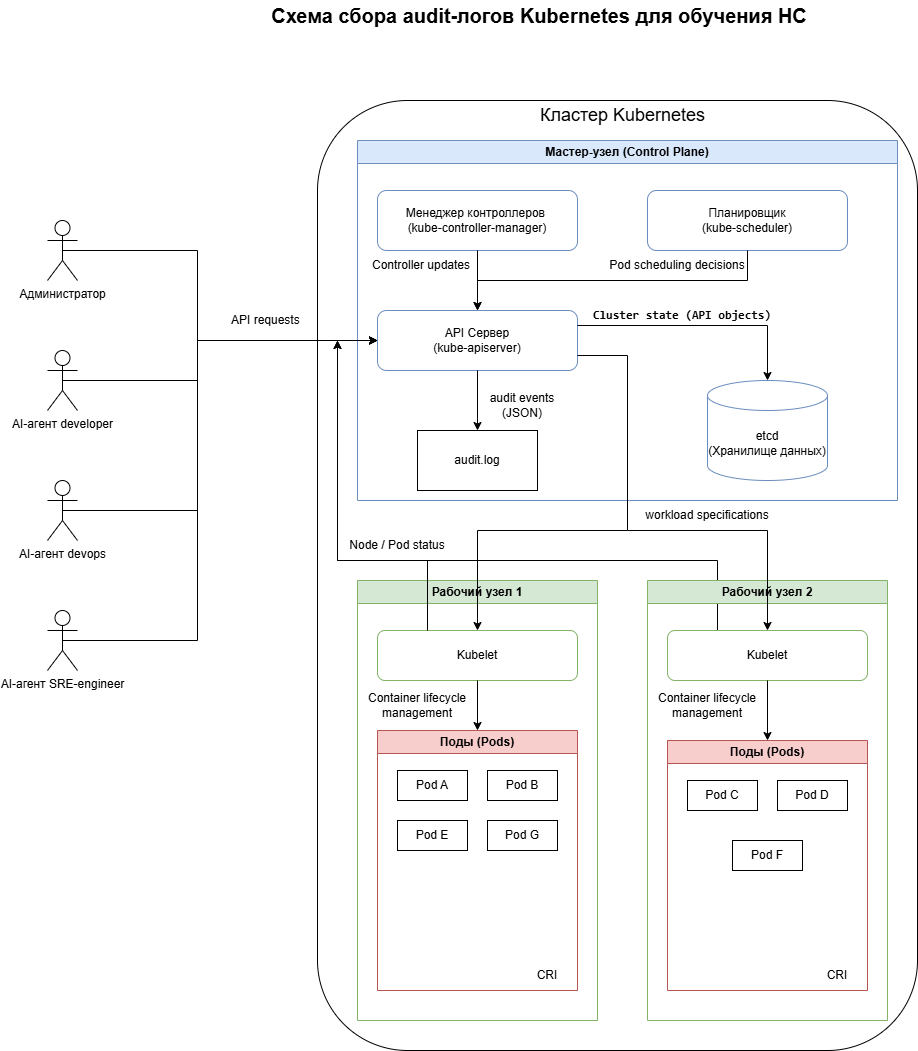
\includegraphics[scale=0.5]{inc/images/cluster-architecture}
    \caption{Архитектура экспериментальной среды}
    \label{fig:cluster_arch}
\end{figure}

Узел плоскости управления выполнял функции управления кластером и включал основные компоненты Kubernetes, такие как \textit{kube-apiserver}, \textit{etcd}, \textit{kube-scheduler} и \textit{kube-controller-manager}. Рабочие узлы использовались для запуска контейнеризированных приложений.

В кластере был включён механизм audit-логирования Kubernetes, фиксирующий все обращения к API-серверу. Конфигурация политики аудита обеспечивала регистрацию основных параметров запросов. Среди них: тип операции, пользователь, ресурс, пространство имён, источник запроса и результат выполнения операции. Audit-логи собирались в процессе взаимодействия пользователей и автоматизированных сервисов с кластером и далее использовались для формирования набора данных, применяемого при обучении и тестировании моделей обнаружения аномалий.

\subsubsection{Генерация событий audit-логов с использованием агентов}

Для генерации событий аудита использовались специализированные агенты-симуляторы поведения, имитирующие типичное поведение различных ролей пользователей в инфраструктуре Kubernetes. Использование агентов позволило автоматически формировать последовательности операций, соответствующие реальным сценариям эксплуатации кластера.

В рамках эксперимента были реализованы три типа агентов:

\begin{itemize}
    \item \textbf{developer} — агент, моделирующий поведение разработчика, взаимодействующего с кластером для развертывания и тестирования приложений. Данный агент выполняет операции создания и обновления Deployment, получения информации о подах, просмотра логов контейнеров и взаимодействия с конфигурационными объектами;
    \item \textbf{devops} — агент, моделирующий действия инженера DevOps, отвечающего за управление инфраструктурой и автоматизацию процессов развертывания. Агент выполняет операции управления ресурсами, масштабирования приложений, обновления конфигураций и мониторинга состояния сервисов;
    \item \textbf{SRE-engineer} — агент, моделирующий деятельность инженера по надёжности сервисов (Site Reliability Engineer). Основные действия включают диагностику проблем, анализ состояния системы, получение метрик, просмотр логов и выполнение административных операций по восстановлению работоспособности сервисов.
\end{itemize}

Каждый агент функционировал на основе заранее заданного профиля поведения, определяющего допустимые типы операций, используемые ресурсы Kubernetes, характерные пространства имён и типичные временные паттерны активности. В результате взаимодействия агентов с кластером формировалась последовательность событий audit-логирования, отражающая нормальное поведение пользователей в системе.

\subsubsection{Формирование обучающей и валидационной выборок}

На первом этапе формирования датасета агенты выполняли только действия, соответствующие их стандартным профилям поведения. В результате формировался набор событий audit-логов, отражающий нормальное функционирование системы и типичное взаимодействие пользователей с кластером.

Полученные события использовались для формирования обучающей и валидационной выборок:

\begin{itemize}
    \item обучающая выборка $\mathcal{X}_{train}$ формировалась из основной части событий нормального поведения и использовалась для обучения параметров моделей нейронных сетей;
    \item валидационная выборка $\mathcal{X}_{val}$ выделялась из той же совокупности событий и применялась для контроля процесса обучения.
\end{itemize}

Поскольку рассматриваемая задача относится к задачам обнаружения аномалий, обучающая выборка преимущественно содержит события нормального поведения. Это позволяет модели сформировать представление о типичных паттернах взаимодействия пользователей с кластером.

\subsubsection{Формирование тестовой выборки и внедрение аномалий}

После формирования обучающей и валидационной выборок была сформирована тестовая выборка $\mathcal{X}_{test}$, предназначенная для оценки качества моделей обнаружения аномалий.

Для этого в профили поведения агентов были встроены дополнительные паттерны взаимодействия с кластером, которые нарушают заданные политики доступа или статистические 
паттерны нормального поведения. Эти действия имитировали аномальное поведение, потенциально связанное с нарушением безопасности или нетипичной активностью пользователя.

К таким паттернам могли относиться:

\begin{itemize}
    \item доступ к нетипичным для роли ресурсам Kubernetes;
    \item выполнение операций, не характерных для конкретного агента;
    \item обращения к чувствительным ресурсам, таким как \texttt{secrets};
    \item нетипичная последовательность операций;
    \item повышенная частота запросов к API-серверу.
\end{itemize}

События, сгенерированные при выполнении таких сценариев, помечались как аномальные. Таким образом, тестовая выборка содержала как нормальные, так и аномальные события, что позволило использовать её для объективной оценки качества моделей обнаружения аномалий.

\subsubsection{Итоговая структура датасета}

В результате проведённого процесса генерации и обработки данных был сформирован размеченный датасет audit-логов Kubernetes, содержащий события нормального и аномального поведения пользователей.

Датасет был разделён на три подмножества:

\begin{itemize}
    \item обучающая выборка $\mathcal{X}_{train}$ --- используется для обучения параметров нейронных сетей;
    \item валидационная выборка $\mathcal{X}_{val}$ --- используется для контроля процесса обучения и настройки гиперпараметров моделей;
    \item тестовая выборка $\mathcal{X}_{test}$ --- содержит размеченные события и используется для итоговой оценки качества моделей обнаружения аномалий.
\end{itemize}

Каждое событие после предобработки представляется в виде вектора признаков фиксированной размерности $x_t \in \mathbb{R}^d$, что обеспечивает возможность применения методов машинного обучения для анализа поведения пользователей и выявления аномалий в Kubernetes-кластере.

\subsubsection{Анализ полученного датасета}

Ниже представлен анализ сформированного датасета audit-логов Kubernetes. Цель анализа --- оценить пригодность данных для обучения моделей обнаружения аномалий, сбалансированность обучающей и тестовой выборок и соответствие распределений заданным профилям агентов. Для тестовой выборки приведён анализ внедрённых аномалий и их типов.

В таблице~\ref{tab:datasets} приведён обзор обучающей, валидационной и тестовой выборок. Число событий и временной диапазон соответствуют сформированным подмножествам $\mathcal{X}_{\mathrm{train}}$, $\mathcal{X}_{val}$ и $\mathcal{X}_{\mathrm{test}}$. Тестовая выборка содержит поле разметки \texttt{label} (0/1) и долю аномальных событий.

\begin{table}[h]
  \centering
  \caption{Сводная таблица обучающей и тестовой выборки}
  \label{tab:datasets}
  \begin{tabularx}{\textwidth}{|p{2.5cm}|r|X|X|p{2cm}|c|}
    \hline
    Датасет & Событий & Начало (время) & Конец (время) & Разметка (label) & Доля аномалий \\ 
    \hline
    $\mathcal{X}_{\mathrm{train}}$ & 140 305 & 2026-02-25 12:33:09 & 2026-03-11 12:29:37 & Нет & --- \\ 
    \hline
    $\mathcal{X}_{\mathrm{train}}$ & 46 768 & 2026-02-25 12:33:09 & 2026-03-11 12:29:37 & Нет & --- \\ 
    \hline
    $\mathcal{X}_{\mathrm{test}}$   & 45 237  & 2026-03-01 16:12:01 & 2026-03-05 16:11:41 & Есть  & 5.31\% \\ 
    \hline
  \end{tabularx}
\end{table}

Для оценки взаимосвязей между категориальными признаками была построена матрица зависимости Крамера, приведенная на рисунке~\ref{fig:cramer_matrix}. Коэффициент Крамера (Cramér’s V) является статистической мерой силы связи между категориальными признаками и принимает значения в диапазоне от 0 до 1. Значения, близкие к нулю, указывают на отсутствие статистической зависимости между признаками, тогда как значения, близкие к единице, свидетельствуют о сильной связи между ними \cite{Cramer1946}.

\begin{figure}
    \centering
    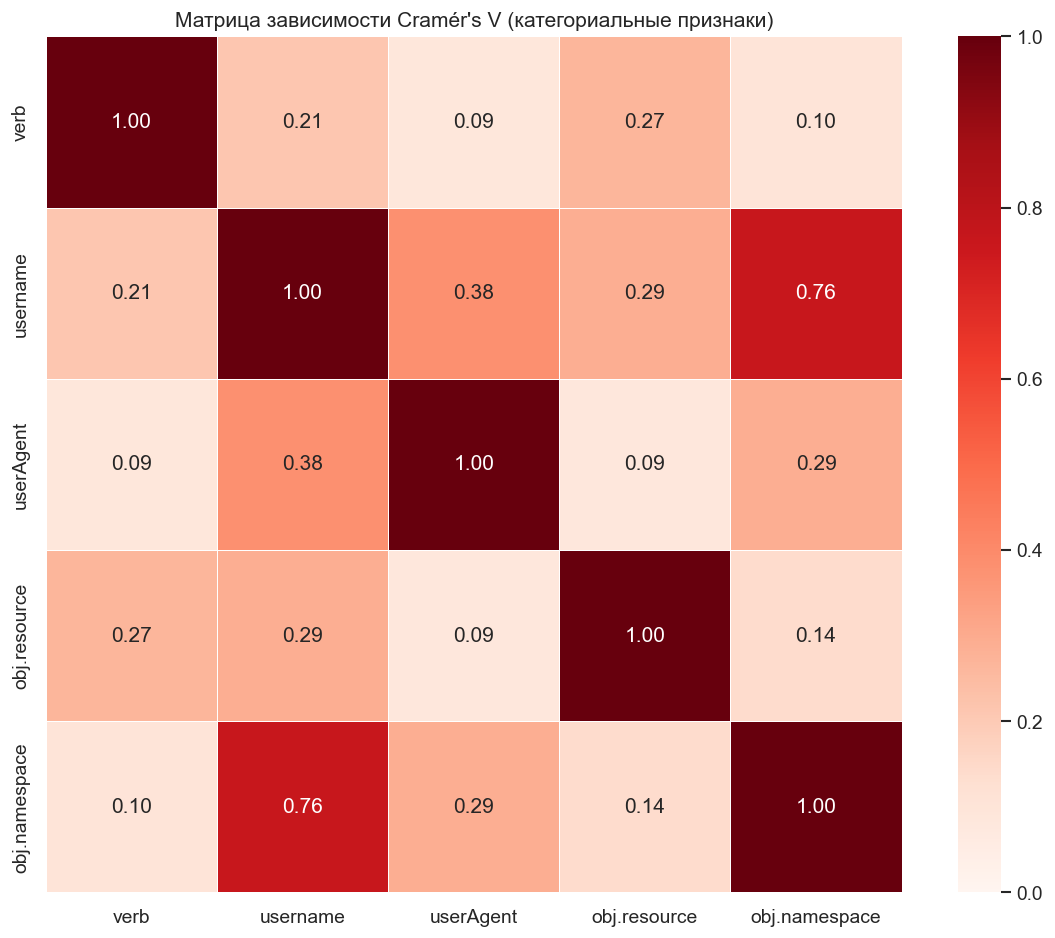
\includegraphics[scale=0.7]{inc/images/cramer_matrix}
    \caption{Матрица зависимости Крамера.}
    \label{fig:cramer_matrix}
\end{figure}

Анализ матрицы зависимости показывает, что большинство признаков характеризуются слабой или умеренной степенью взаимосвязи. Это является ожидаемым результатом для аудит-логов Kubernetes, поскольку различные параметры события формируются независимо и отражают разные аспекты взаимодействия пользователя или компонента системы с API-сервером.

Наиболее сильная зависимость наблюдается между признаками \texttt{username} и \texttt{obj.namespace}, значение коэффициента Крамера для данной пары составляет 0.76. Это указывает на то, что конкретные пользователи или сервисные аккаунты чаще всего взаимодействуют с ограниченным набором пространств имён. Такое поведение соответствует модели разграничения доступа Kubernetes (RBAC), при которой пользователи и сервисные аккаунты обычно имеют доступ только к определённым пространствам имён.

Умеренная зависимость наблюдается между признаками \texttt{username} и \texttt{userAgent} (0.38). Это может быть связано с тем, что различные пользователи или автоматизированные процессы используют характерные клиенты для взаимодействия с API Kubernetes, например утилиту \texttt{kubectl}, CI/CD системы или встроенные компоненты кластера.

\subsection{Разработка и обучение моделей нейронных сетей для обнаружения аномалий}

На основе подготовленных данных разрабатываются модели нейронных сетей, предназначенные для обнаружения аномалий в поведении пользователей и сервисных аккаунтов Kubernetes-кластера.

Для каждой архитектуры выполняется обучение модели на обучающей выборке и настройка её параметров с использованием валидационной выборки. Процесс обучения направлен на минимизацию функции потерь, характеризующей способность модели корректно описывать нормальное поведение пользователей и выявлять аномальные события.

Для достижения этой цели рассматриваются три класса нейронных сетей:

\begin{itemize}
    \item Автокодировщики (Autoencoder, AE).
    \item Рекуррентные нейронные сети (RNN) на основе Autoencoder.
    \item Долгосрочная краткосрочная память (LSTM) на основе Autoencoder.
\end{itemize}

\subsubsection{Autoencoder}

В данной работе автокодировщик используется для обнаружения аномалий в событиях audit-логов Kubernetes. После предобработки каждое событие представляется вектором признаков $x \in \mathbb{R}^d$, который подаётся на вход модели. Автокодировщик обучается восстанавливать нормальные события.

Основная идея заключается в том, что модель хорошо реконструирует только данные, соответствующие распределению обучающей выборки. Аномальные события отличаются от нормального поведения, поэтому ошибка их реконструкции выше.

Функция потерь, используемая при обучении модели, определяется среднеквадратичной ошибкой, представленной в формуле~\ref{eq:mse_loss}.

\begin{equation}\label{eq:mse_loss}
    \mathcal{L}_{MSE} = \frac{1}{d} \| x_i - \tilde{x}_i \|_2^2
\end{equation}

После обучения модели для каждого события вычисляется показатель аномальности, определённый в формуле~\ref{eq:anomaly_score}.

\begin{equation}\label{eq:anomaly_score}
    s_i = \| x_i - \tilde{x}_i \|_2^2
\end{equation}

Чем выше значение $s_i$, тем сильнее событие отклоняется от нормального поведения.

Для обучения автокодировщика используется обучающая выборка $\mathcal{X}_{train}$, содержащая события нормального поведения пользователей Kubernetes-кластера. Валидационная выборка $\mathcal{X}_{val}$ применяется для контроля процесса обучения и предотвращения переобучения. Обучение выполняется итерационно с использованием алгоритма обратного распространения ошибки. На каждой эпохе вычисляется значение функции потерь на обучающей и валидационной выборках, что позволяет отслеживать динамику обучения модели.

Для оптимизации параметров сети используется адаптивный градиентный метод оптимизации Adam, обеспечивающий устойчивую и быструю сходимость. В процессе обучения применяются методы регуляризации, такие как Dropout и ранняя остановка (Early Stopping).

На рисунке~\ref{fig:ae_training_loss} представлен график изменения функции потерь на обучающей и валидационной выборках.

\begin{figure}
    \centering
    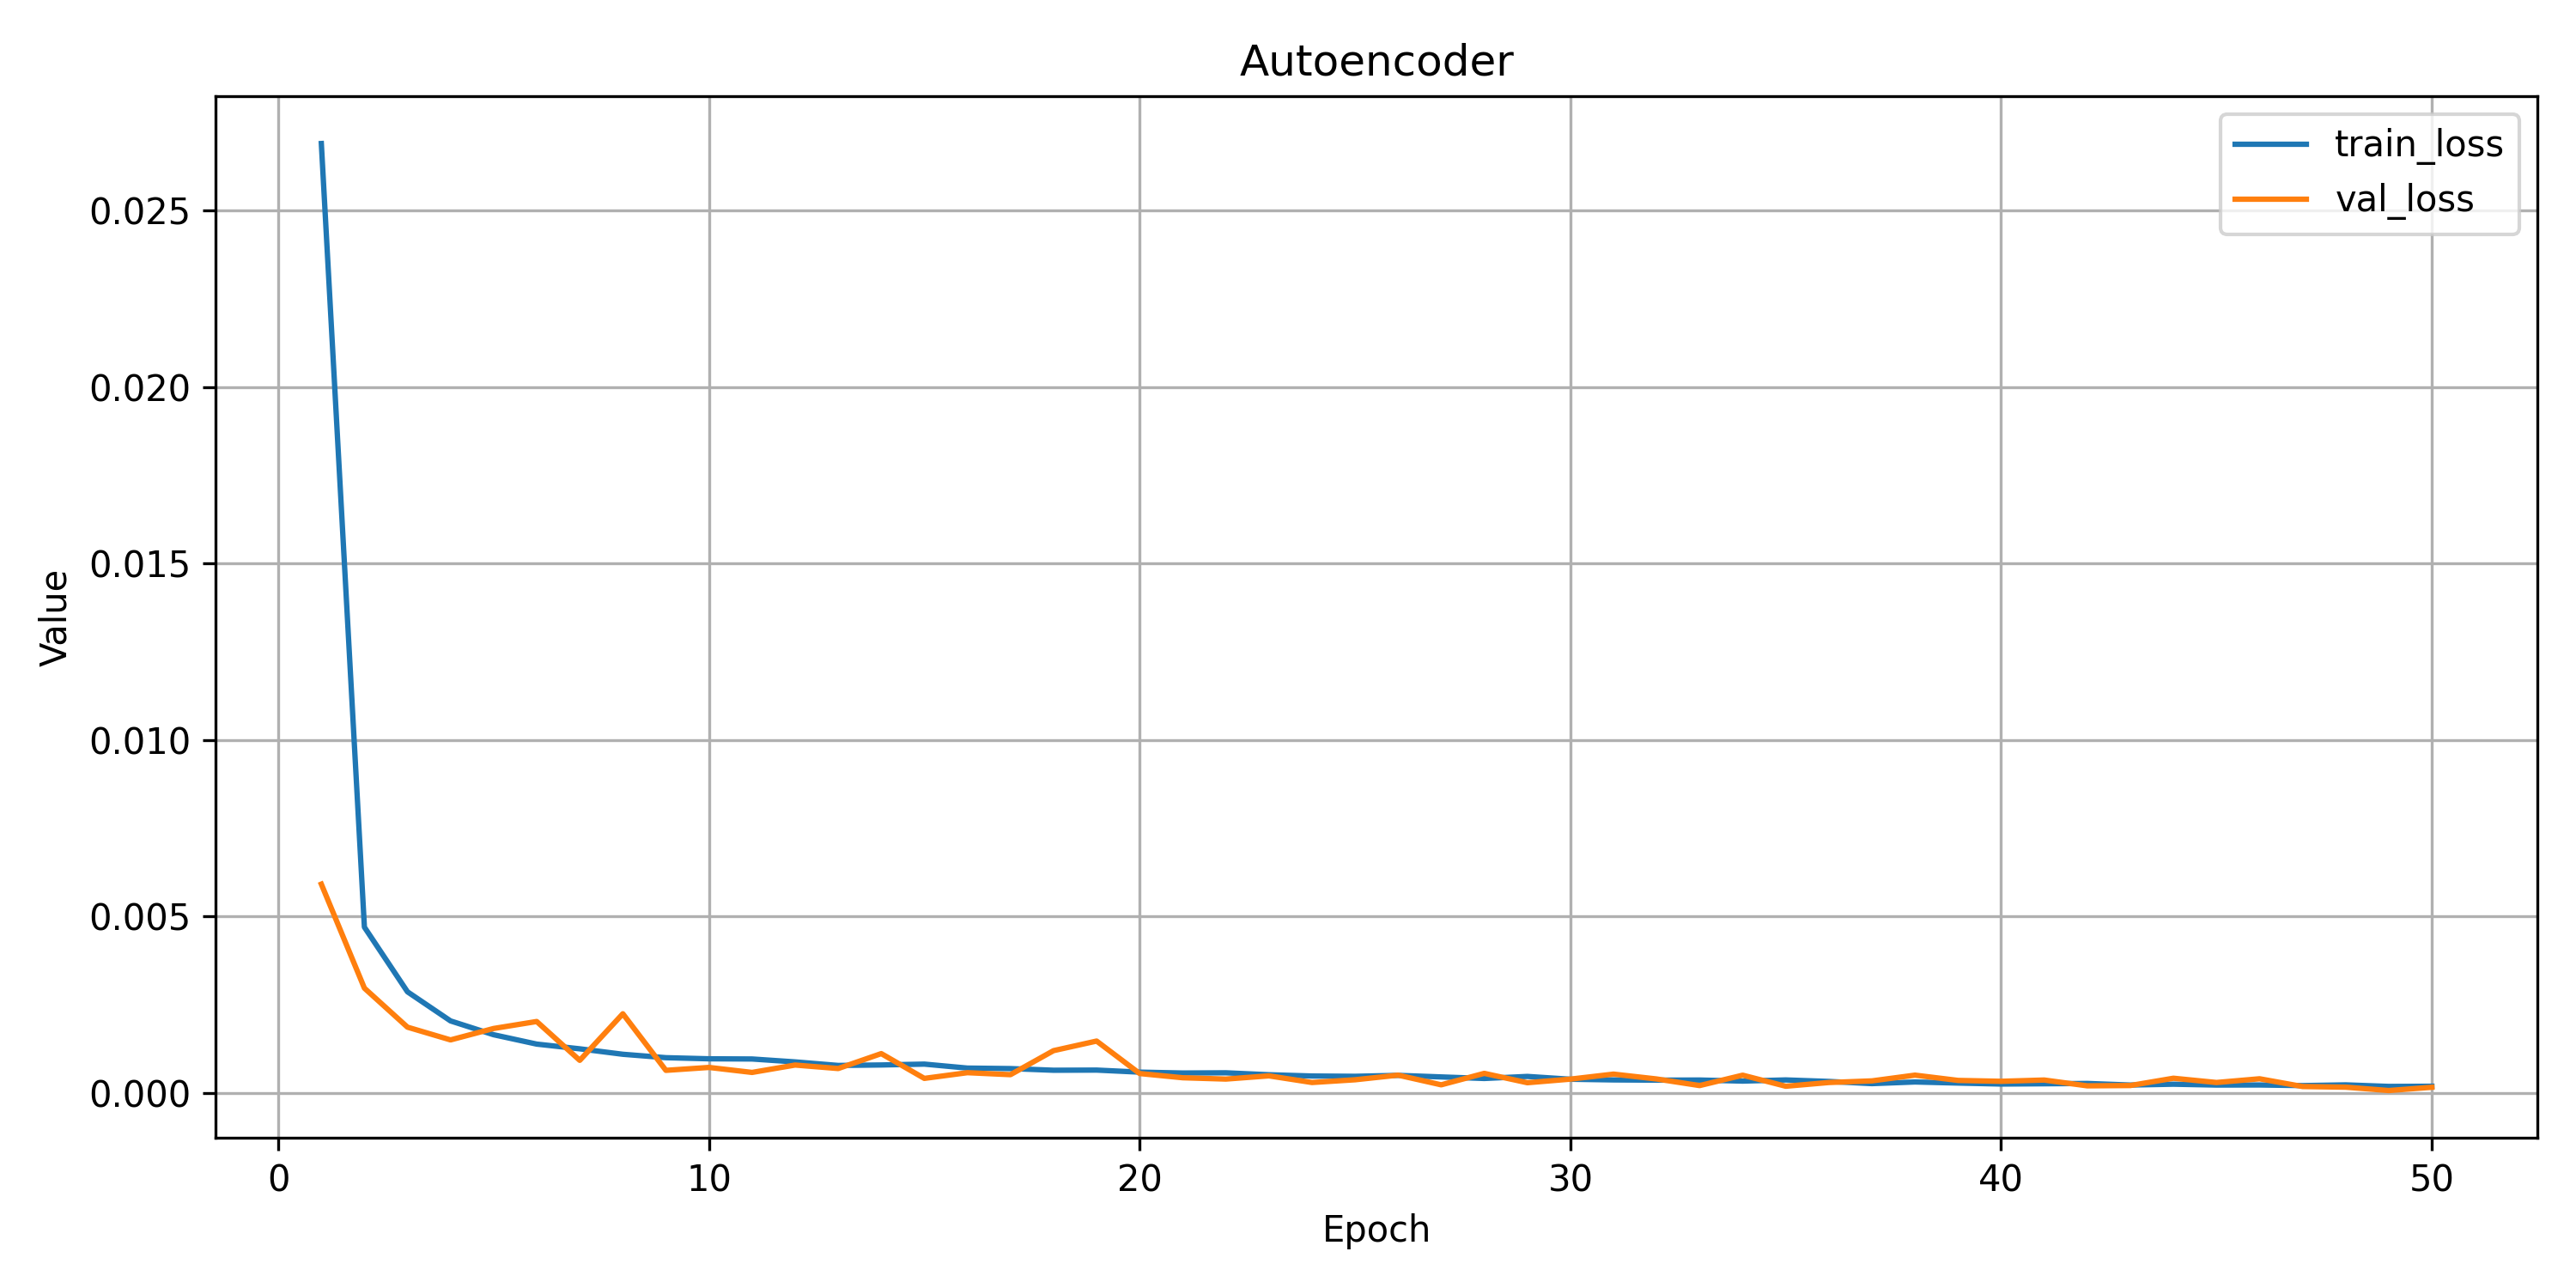
\includegraphics[scale=0.7]{inc/images/ae_training_loss}
    \caption{Изменение функции потерь Autoencoder в процессе обучения.}
    \label{fig:ae_training_loss}
\end{figure}

После завершения обучения для событий тестовой выборки $\mathcal{X}_{test}$ вычисляется ошибка реконструкции. Для разделения нормальных и аномальных событий вводится пороговое значение $\tau$, как показано в формуле ~\ref{eq:anomaly_score_y}.

\begin{equation}\label{eq:anomaly_score_y}
    y_i =
    \begin{cases}
        1, & \text{если } s_i > \tau,\\
        0, & \text{иначе}.
    \end{cases}
\end{equation}

На рисунке~\ref{fig:ae_reconstruction_error} показано распределение ошибки реконструкции для нормальных и аномальных событий.

\begin{figure}
    \centering
    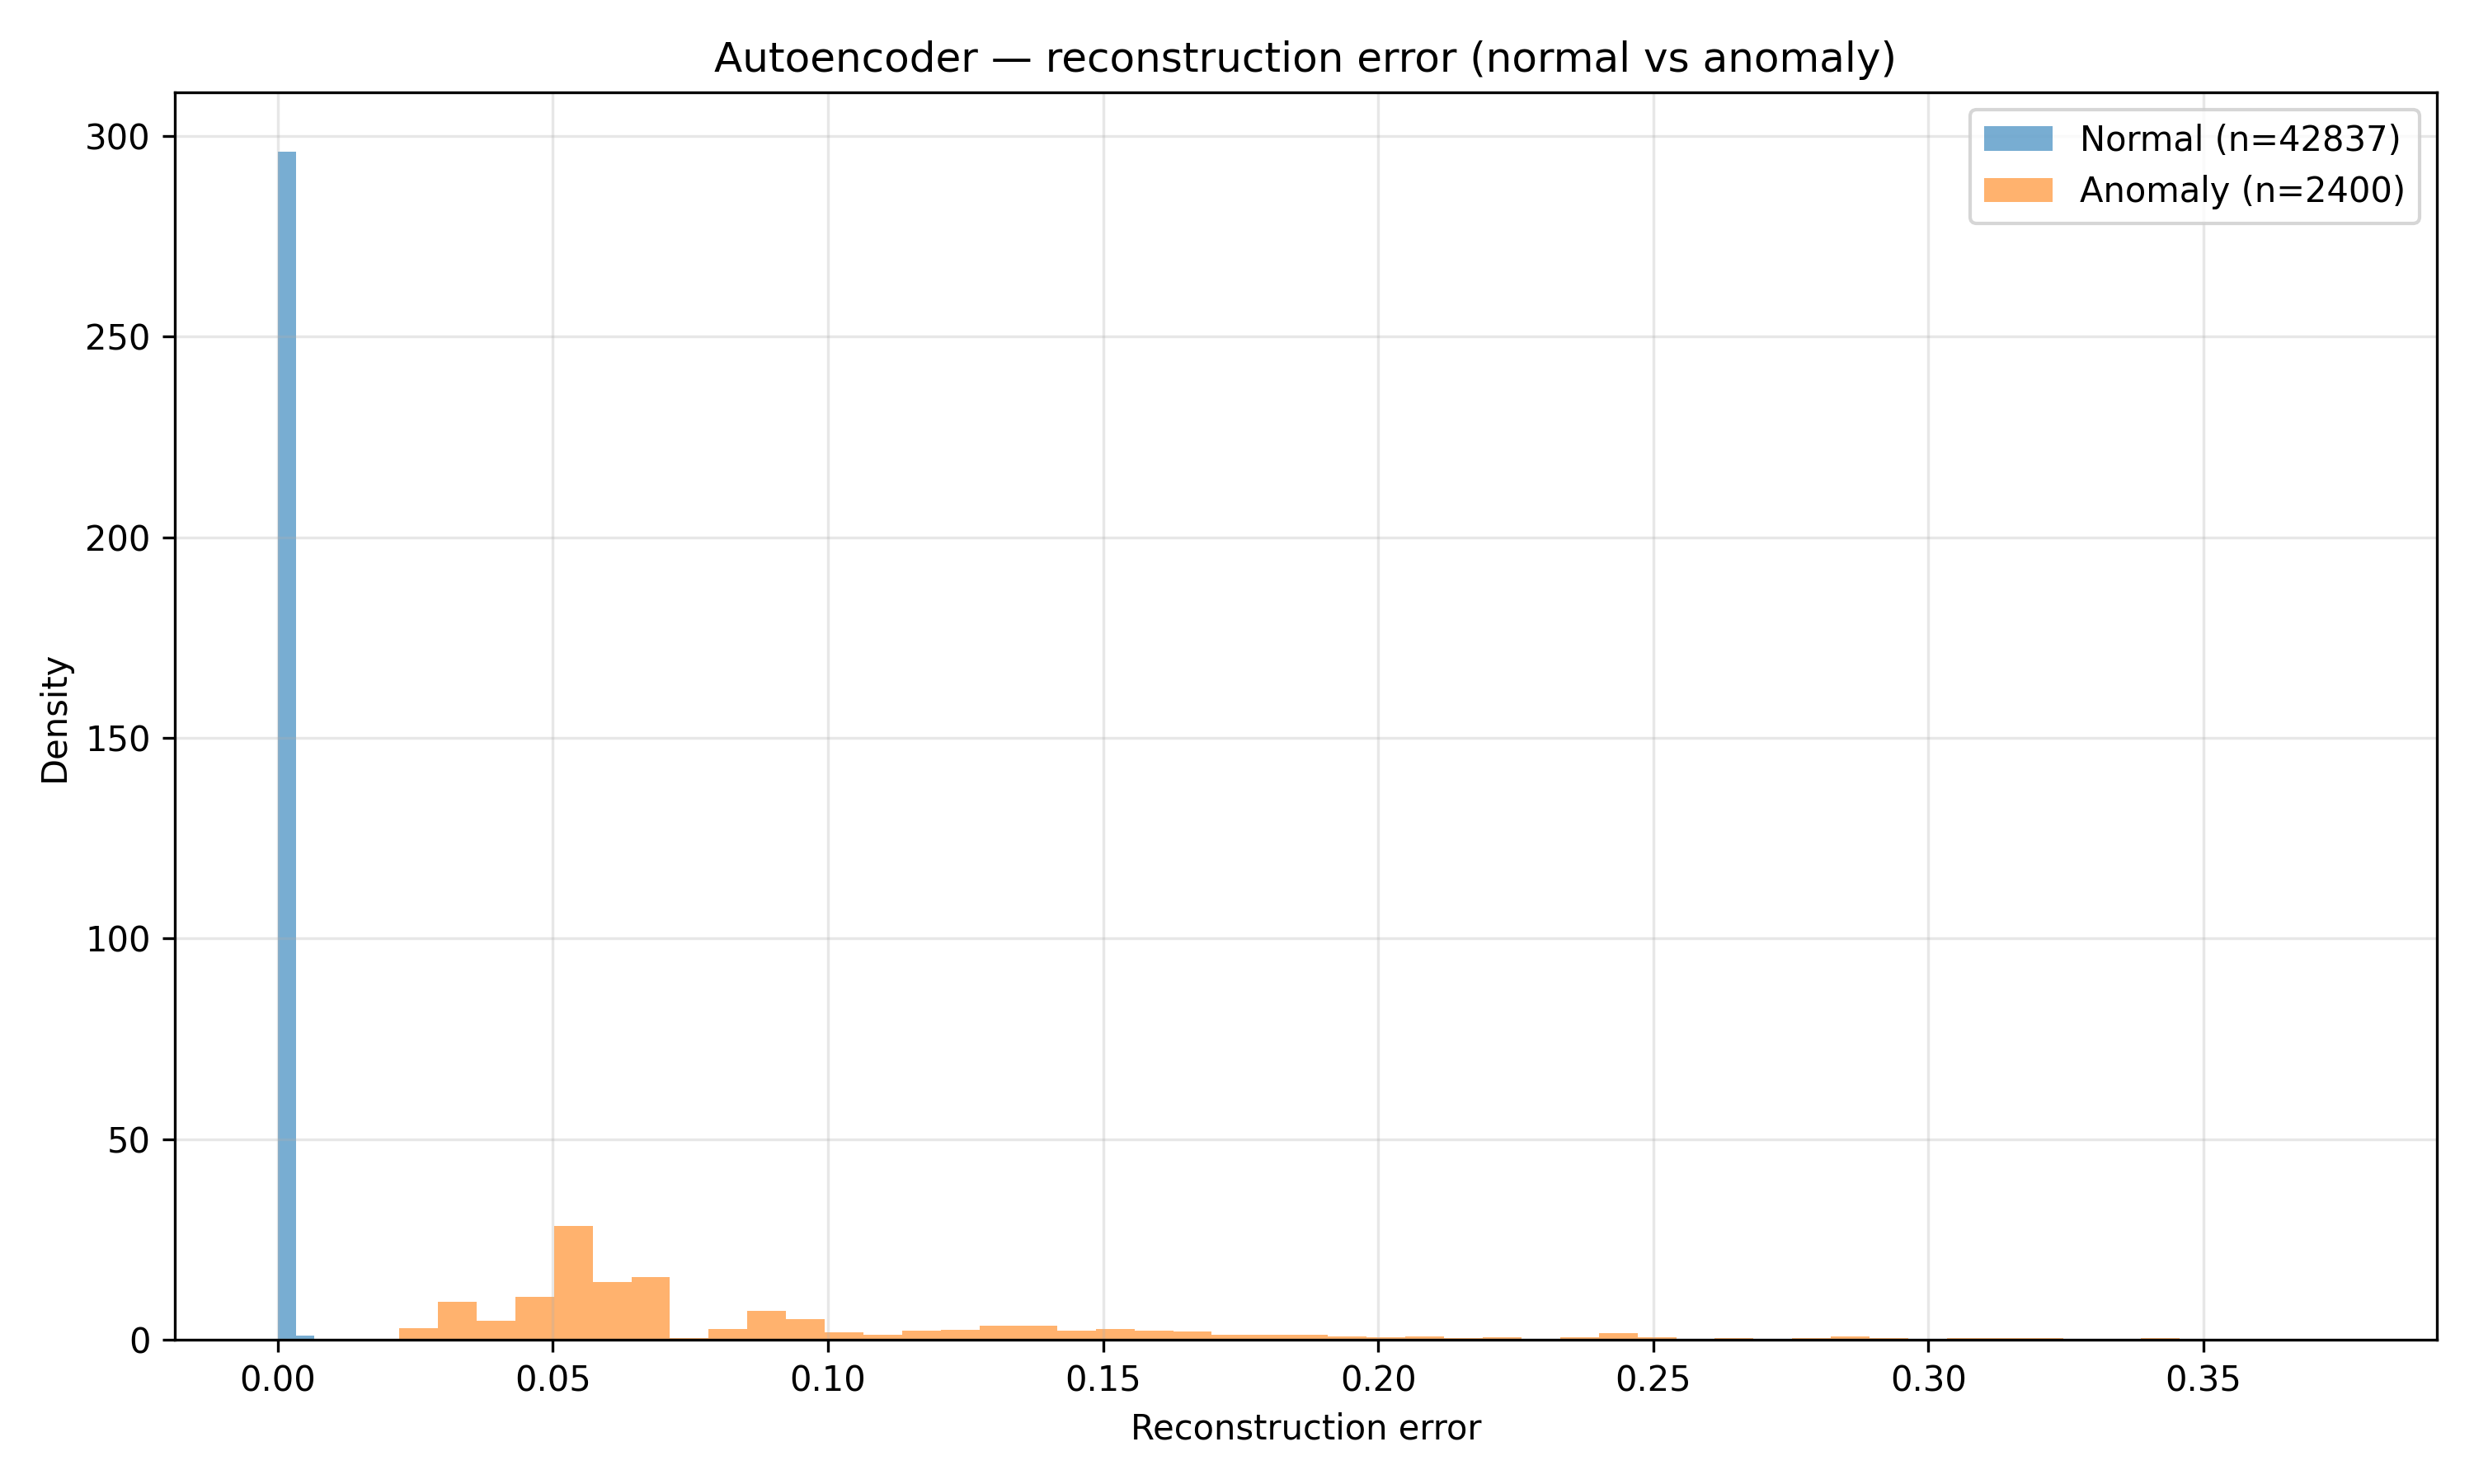
\includegraphics[scale=0.7]{inc/images/ae_reconstruction_error}
    \caption{Распределение ошибки реконструкции для модели Autoencoder.}
    \label{fig:ae_reconstruction_error}
\end{figure}

Для количественной оценки качества обнаружения аномалий используется метрика площади под PR-кривой (PR-AUC), является предпочтительной при сильном дисбалансе классов.

На рисунке~\ref{fig:ae_pr_curve} представлена PR-кривая для модели Autoencoder.

\begin{figure}
    \centering
    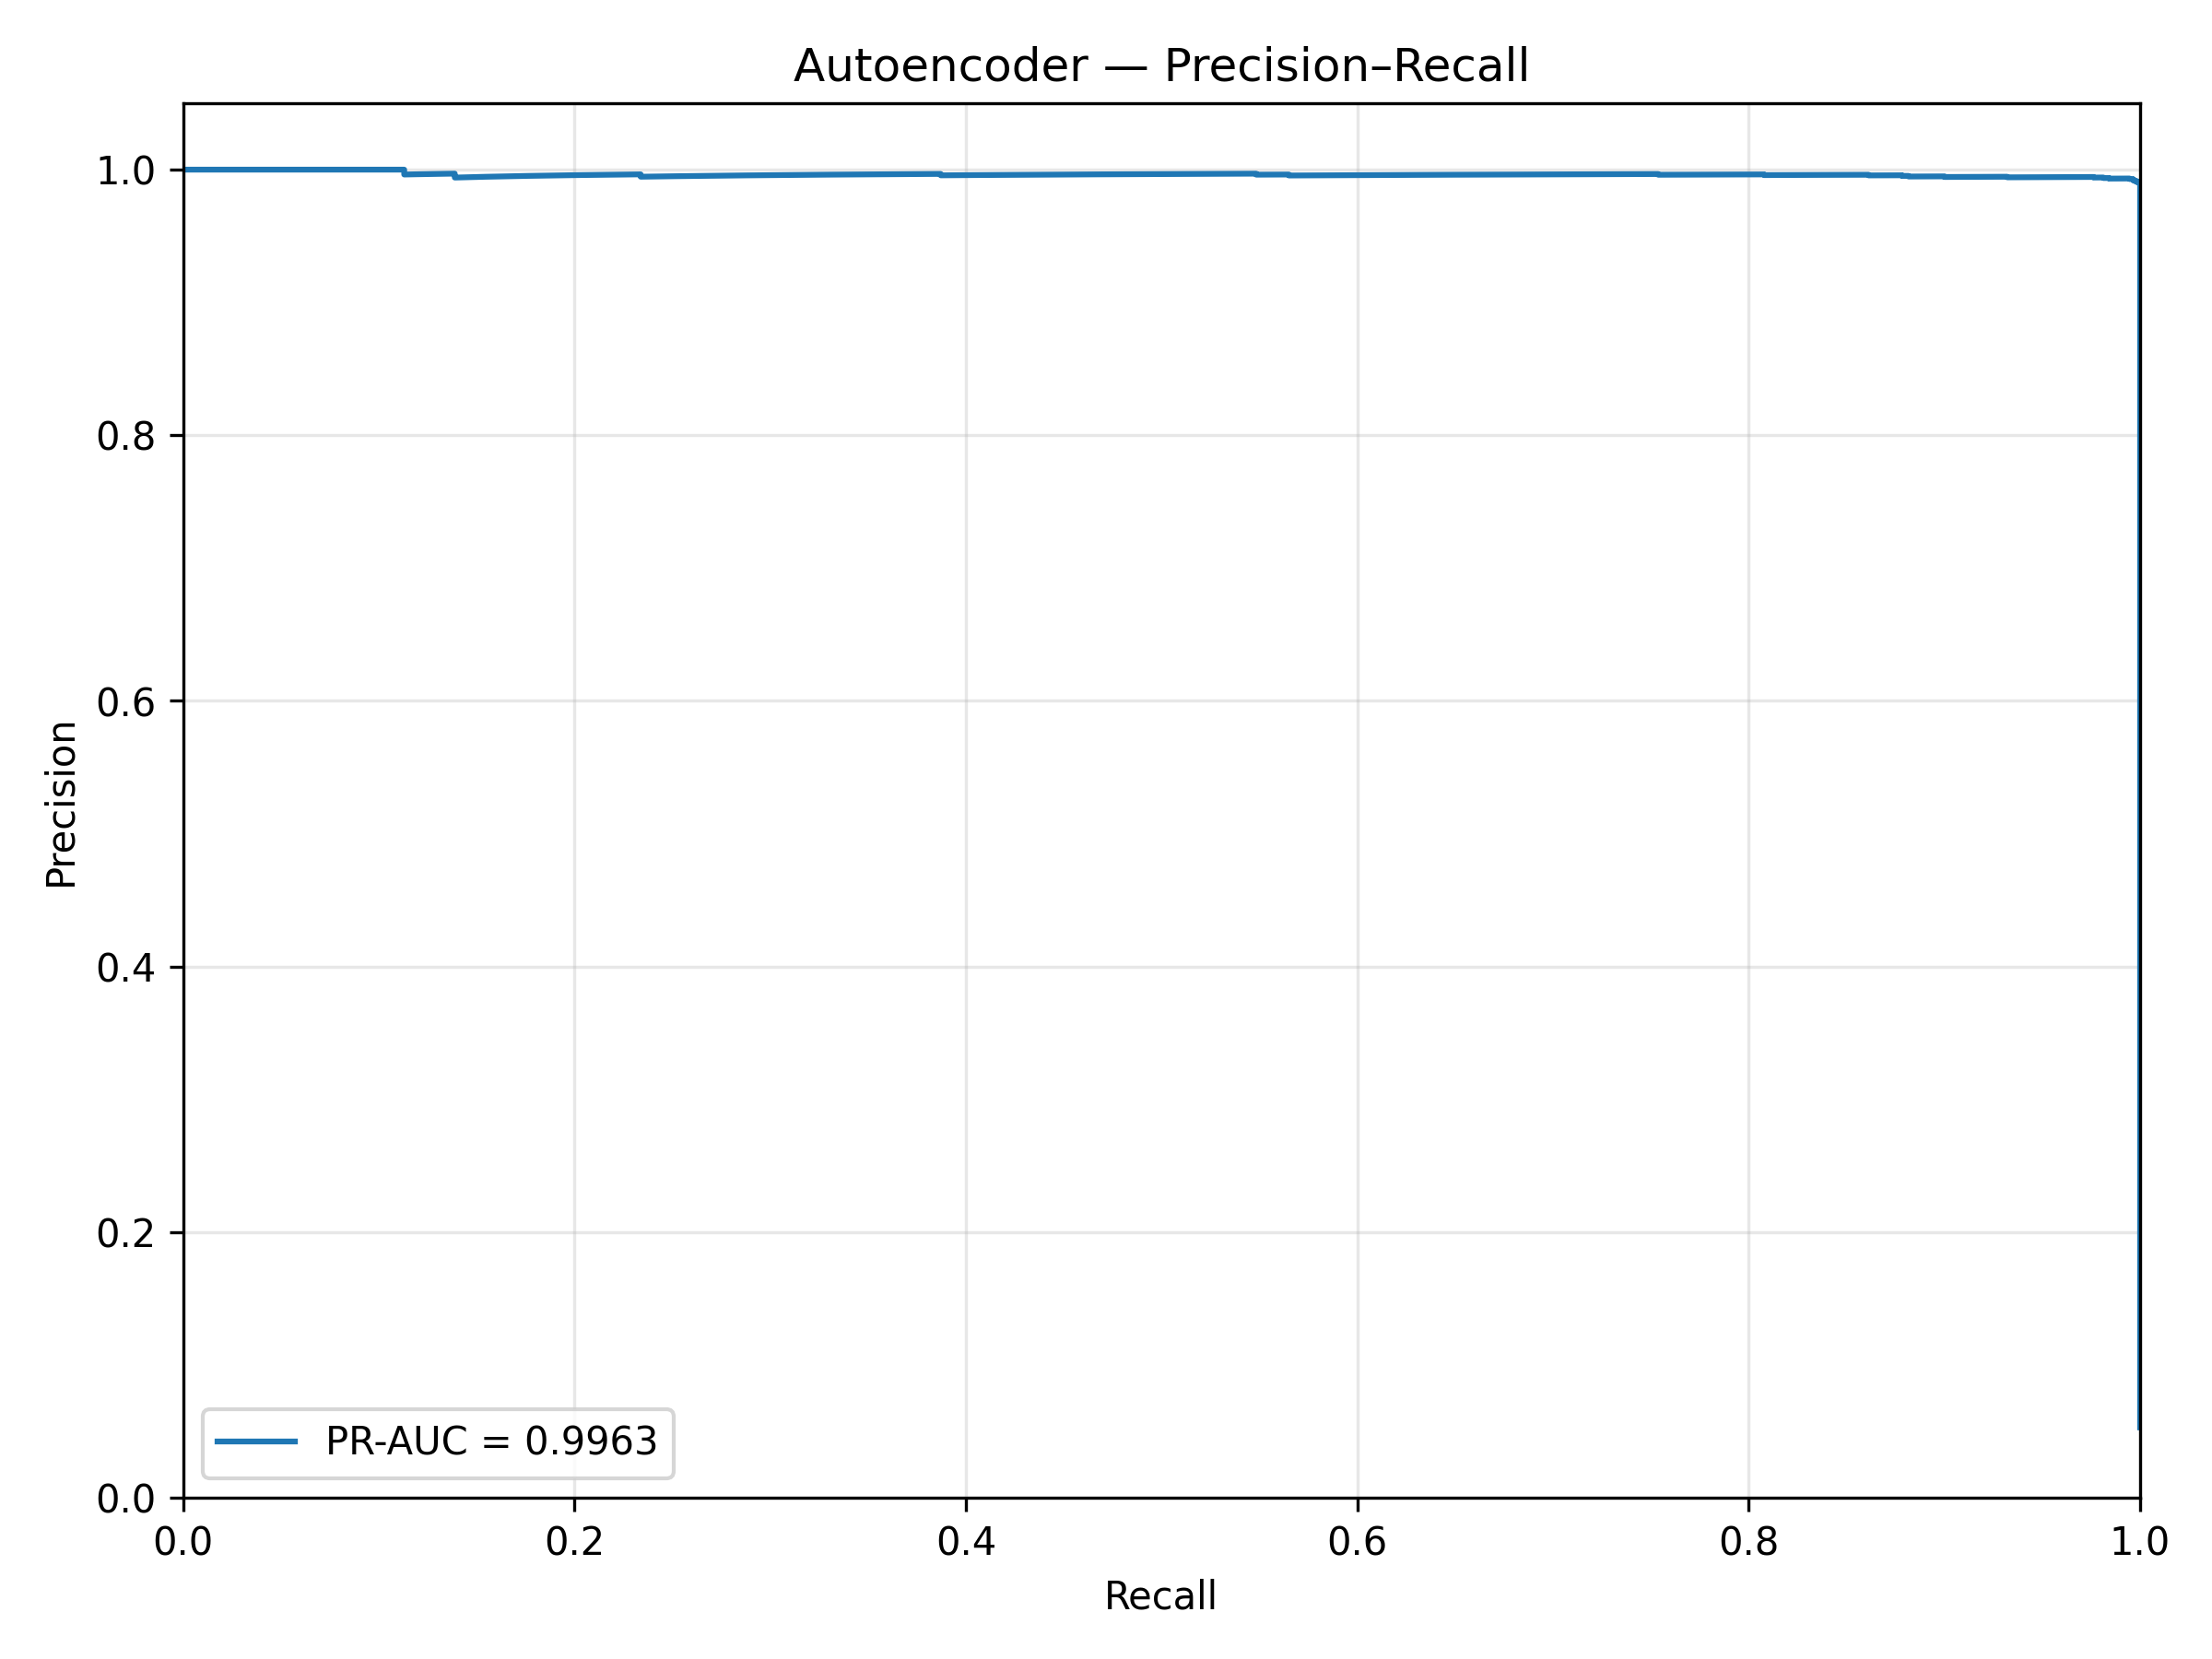
\includegraphics[scale=0.7]{inc/images/ae_pr_curve}
    \caption{PR-кривая для модели Autoencoder.}
    \label{fig:ae_pr_curve}
\end{figure}

\subsubsection{RNN-Autoencoder}

В данной работе RNN используется в архитектуре \textit{autoencoder} (RNN-AE), где слои \textit{encoder} и \textit{decoder} состоят из RNN-блоков. Такая структура позволяет моделировать последовательности событий audit-логов и выявлять аномалии, связанные с нетипичным поведением пользователей или сервисных аккаунтов.

На рисунке~\ref{fig:RNN-AE} приведена архитектура RNN-Autoencoder, состоящая из двух частей:
\begin{itemize}
    \item \textbf{Encoder} — один или несколько RNN-слоёв, преобразующих последовательность входных векторов $x_t$ в фиксированный вектор контекста $z$, содержащий сводную информацию о последовательности событий;
    \item \textbf{Decoder} — RNN-слои, которые на основе вектора $z$ восстанавливают исходную последовательность событий $\tilde{x}_t$.
\end{itemize}

\begin{figure}
    \centering
    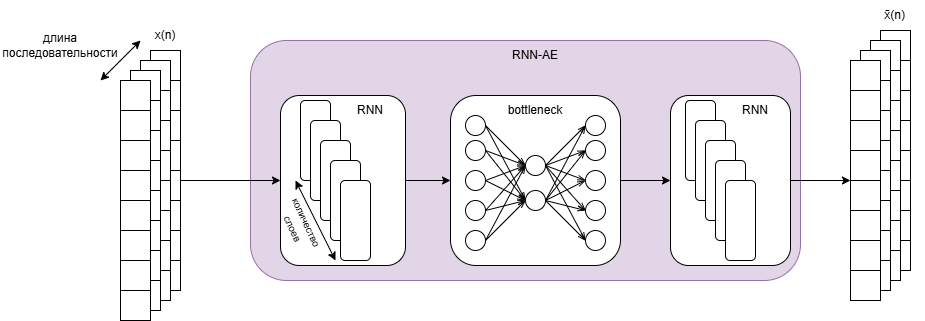
\includegraphics[scale=0.45]{inc/images/RNN-AE-architecture}
    \caption{Архитектура RNN-Autoencoder.}
    \label{fig:RNN-AE}
\end{figure}

Функция потерь, используемая для обучения модели, определяется среднеквадратичной ошибкой, представленной в формуле~\ref{eq:rnn_mse}.

\nopagebreak
\begin{equation}\label{eq:rnn_mse}
    \mathcal{L}_{MSE} = \frac{1}{T} \sum_{t=1}^{T} \frac{1}{d} \| x_it - \tilde{x}_it \|_2^2
\end{equation}

где $T$ - длина последовательности, подающаяся в модель.

После обучения модели показатель аномальности вычисляется по формуле~\ref{eq:rnn_score}.

\begin{equation}\label{eq:rnn_score}
    s_t = \frac{1}{T} \sum_{t=1}^{T} \| x_it - \tilde{x}_it \|_2^2
\end{equation}

где $s_t$ — показатель аномальности для события $t$. События с $s_t$, превышающим пороговое значение, считаются аномальными.

На рисунке~\ref{fig:rnn_training_loss} представлен график изменения функции потерь модели RNN-AE на обучающей и валидационной выборках.

\begin{figure}
    \centering
    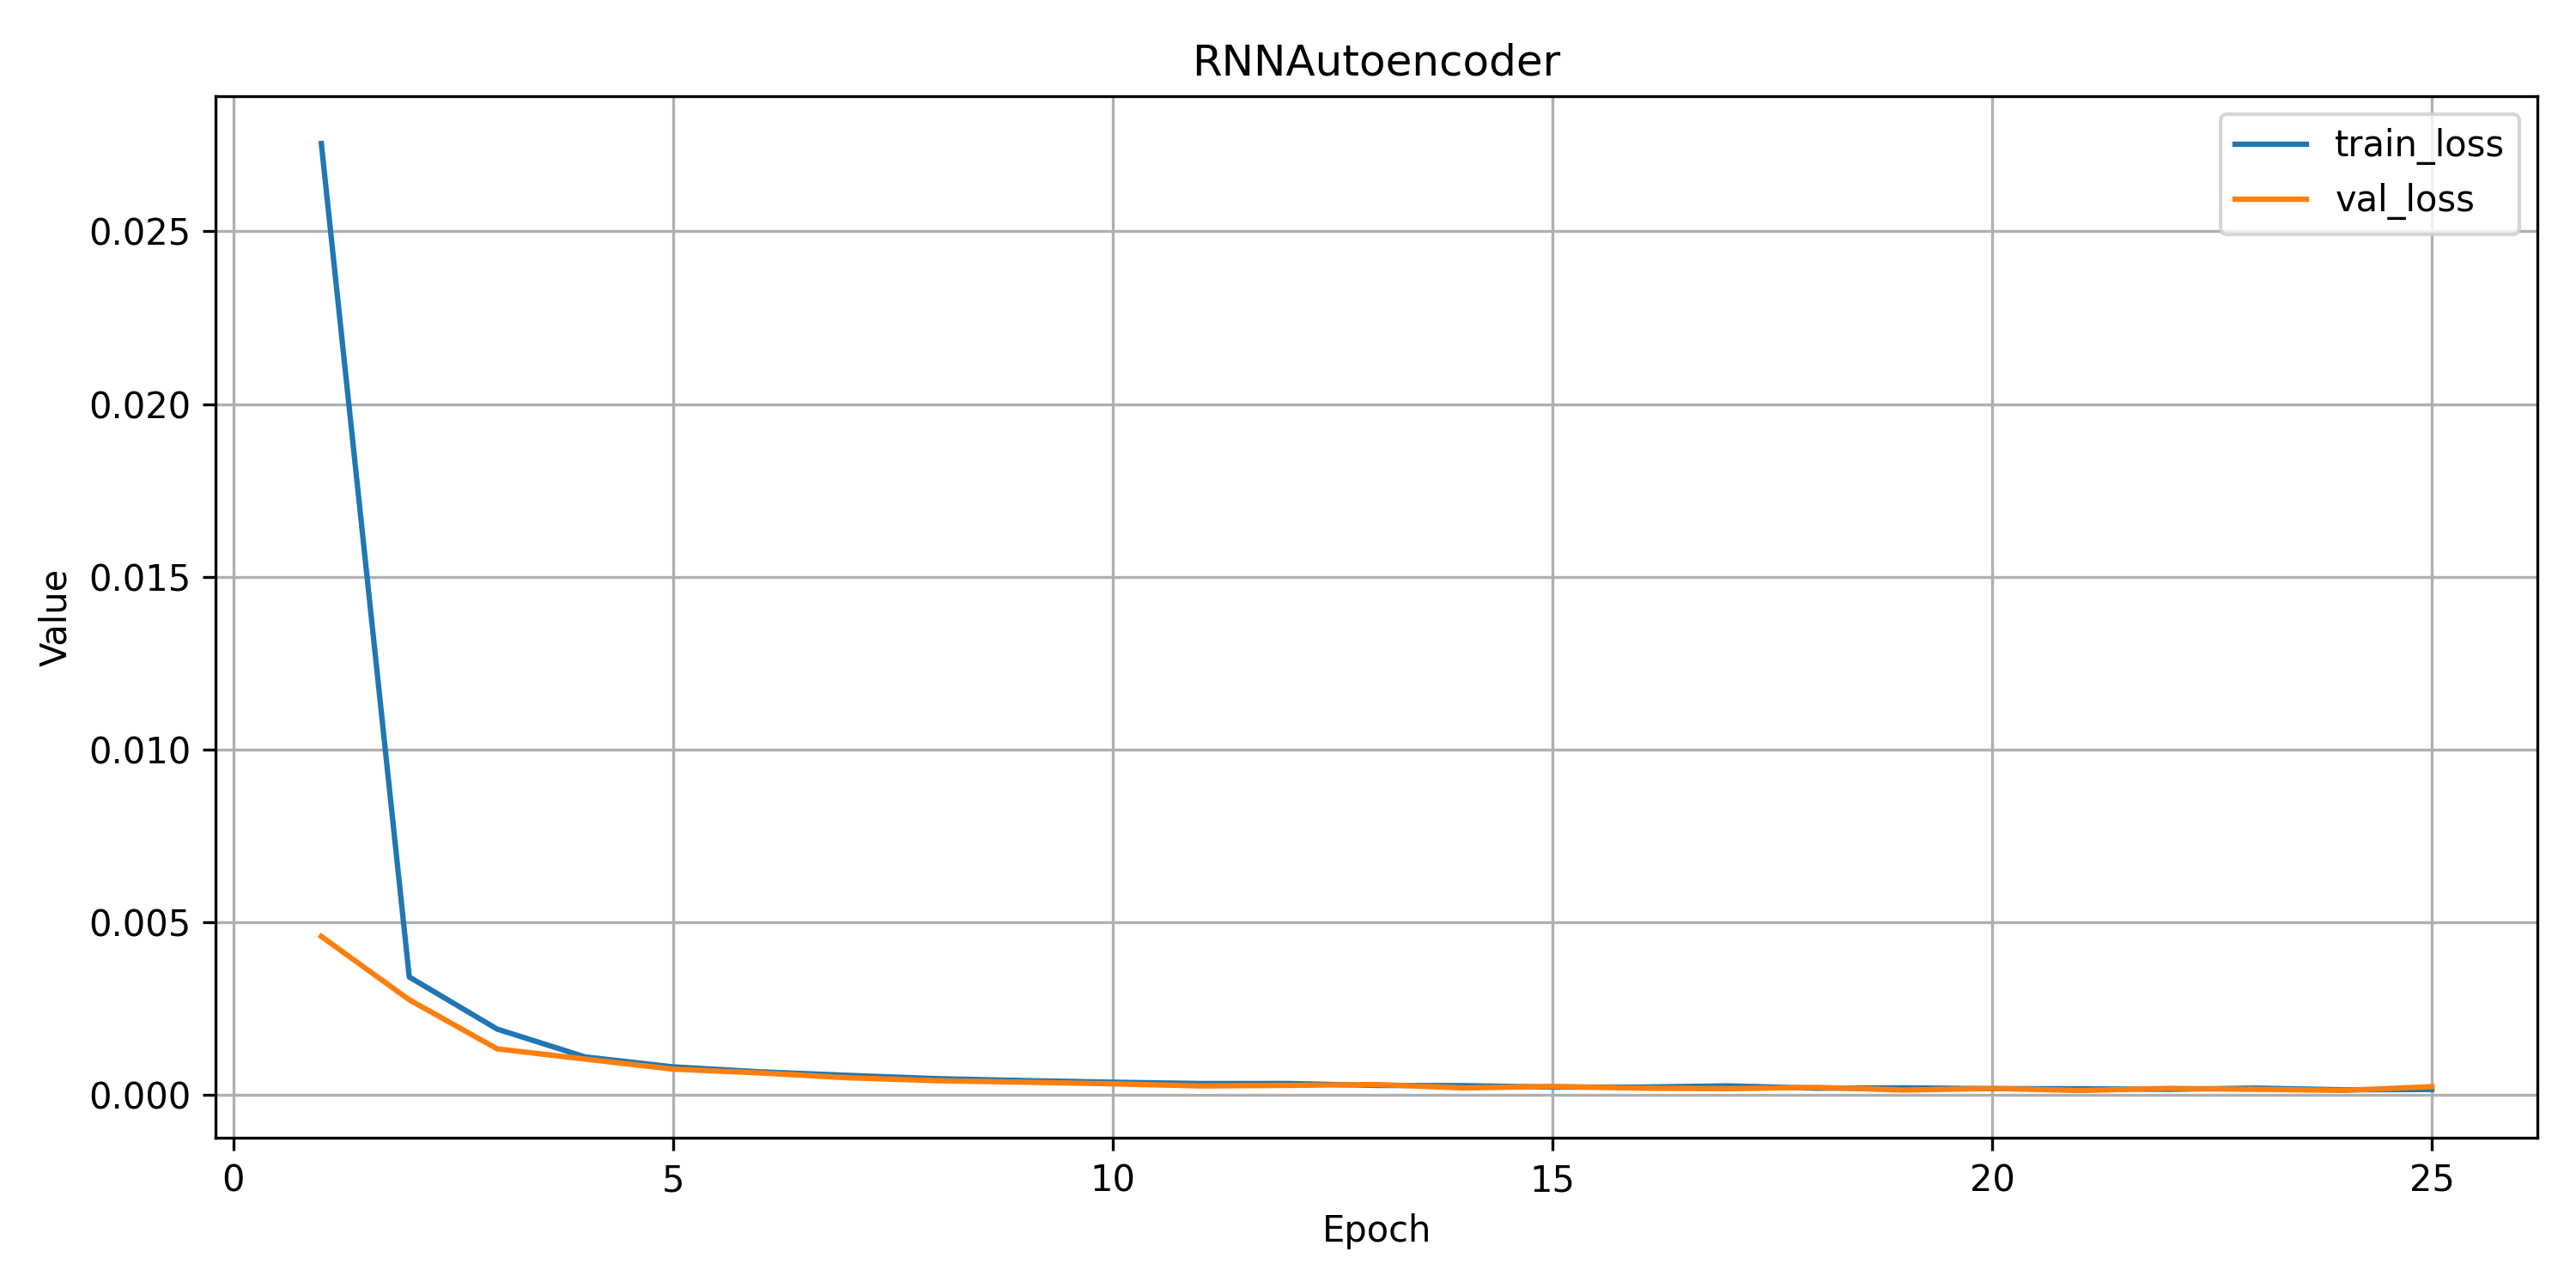
\includegraphics[scale=0.7]{inc/images/rnn_training_loss}
    \caption{Изменение функции потерь модели RNN-AE в процессе обучения.}
    \label{fig:rnn_training_loss}
\end{figure}

После завершения обучения для каждого события тестовой выборки вычисляется показатель аномальности $s_t$, основанный на величине ошибки реконструкции.

На рисунке~\ref{fig:rnn_reconstruction_error} показано распределение ошибки реконструкции для нормальных и аномальных событий. Как правило, аномальные события характеризуются более высокими значениями ошибки, что позволяет использовать этот показатель для их обнаружения.

\begin{figure}
    \centering
    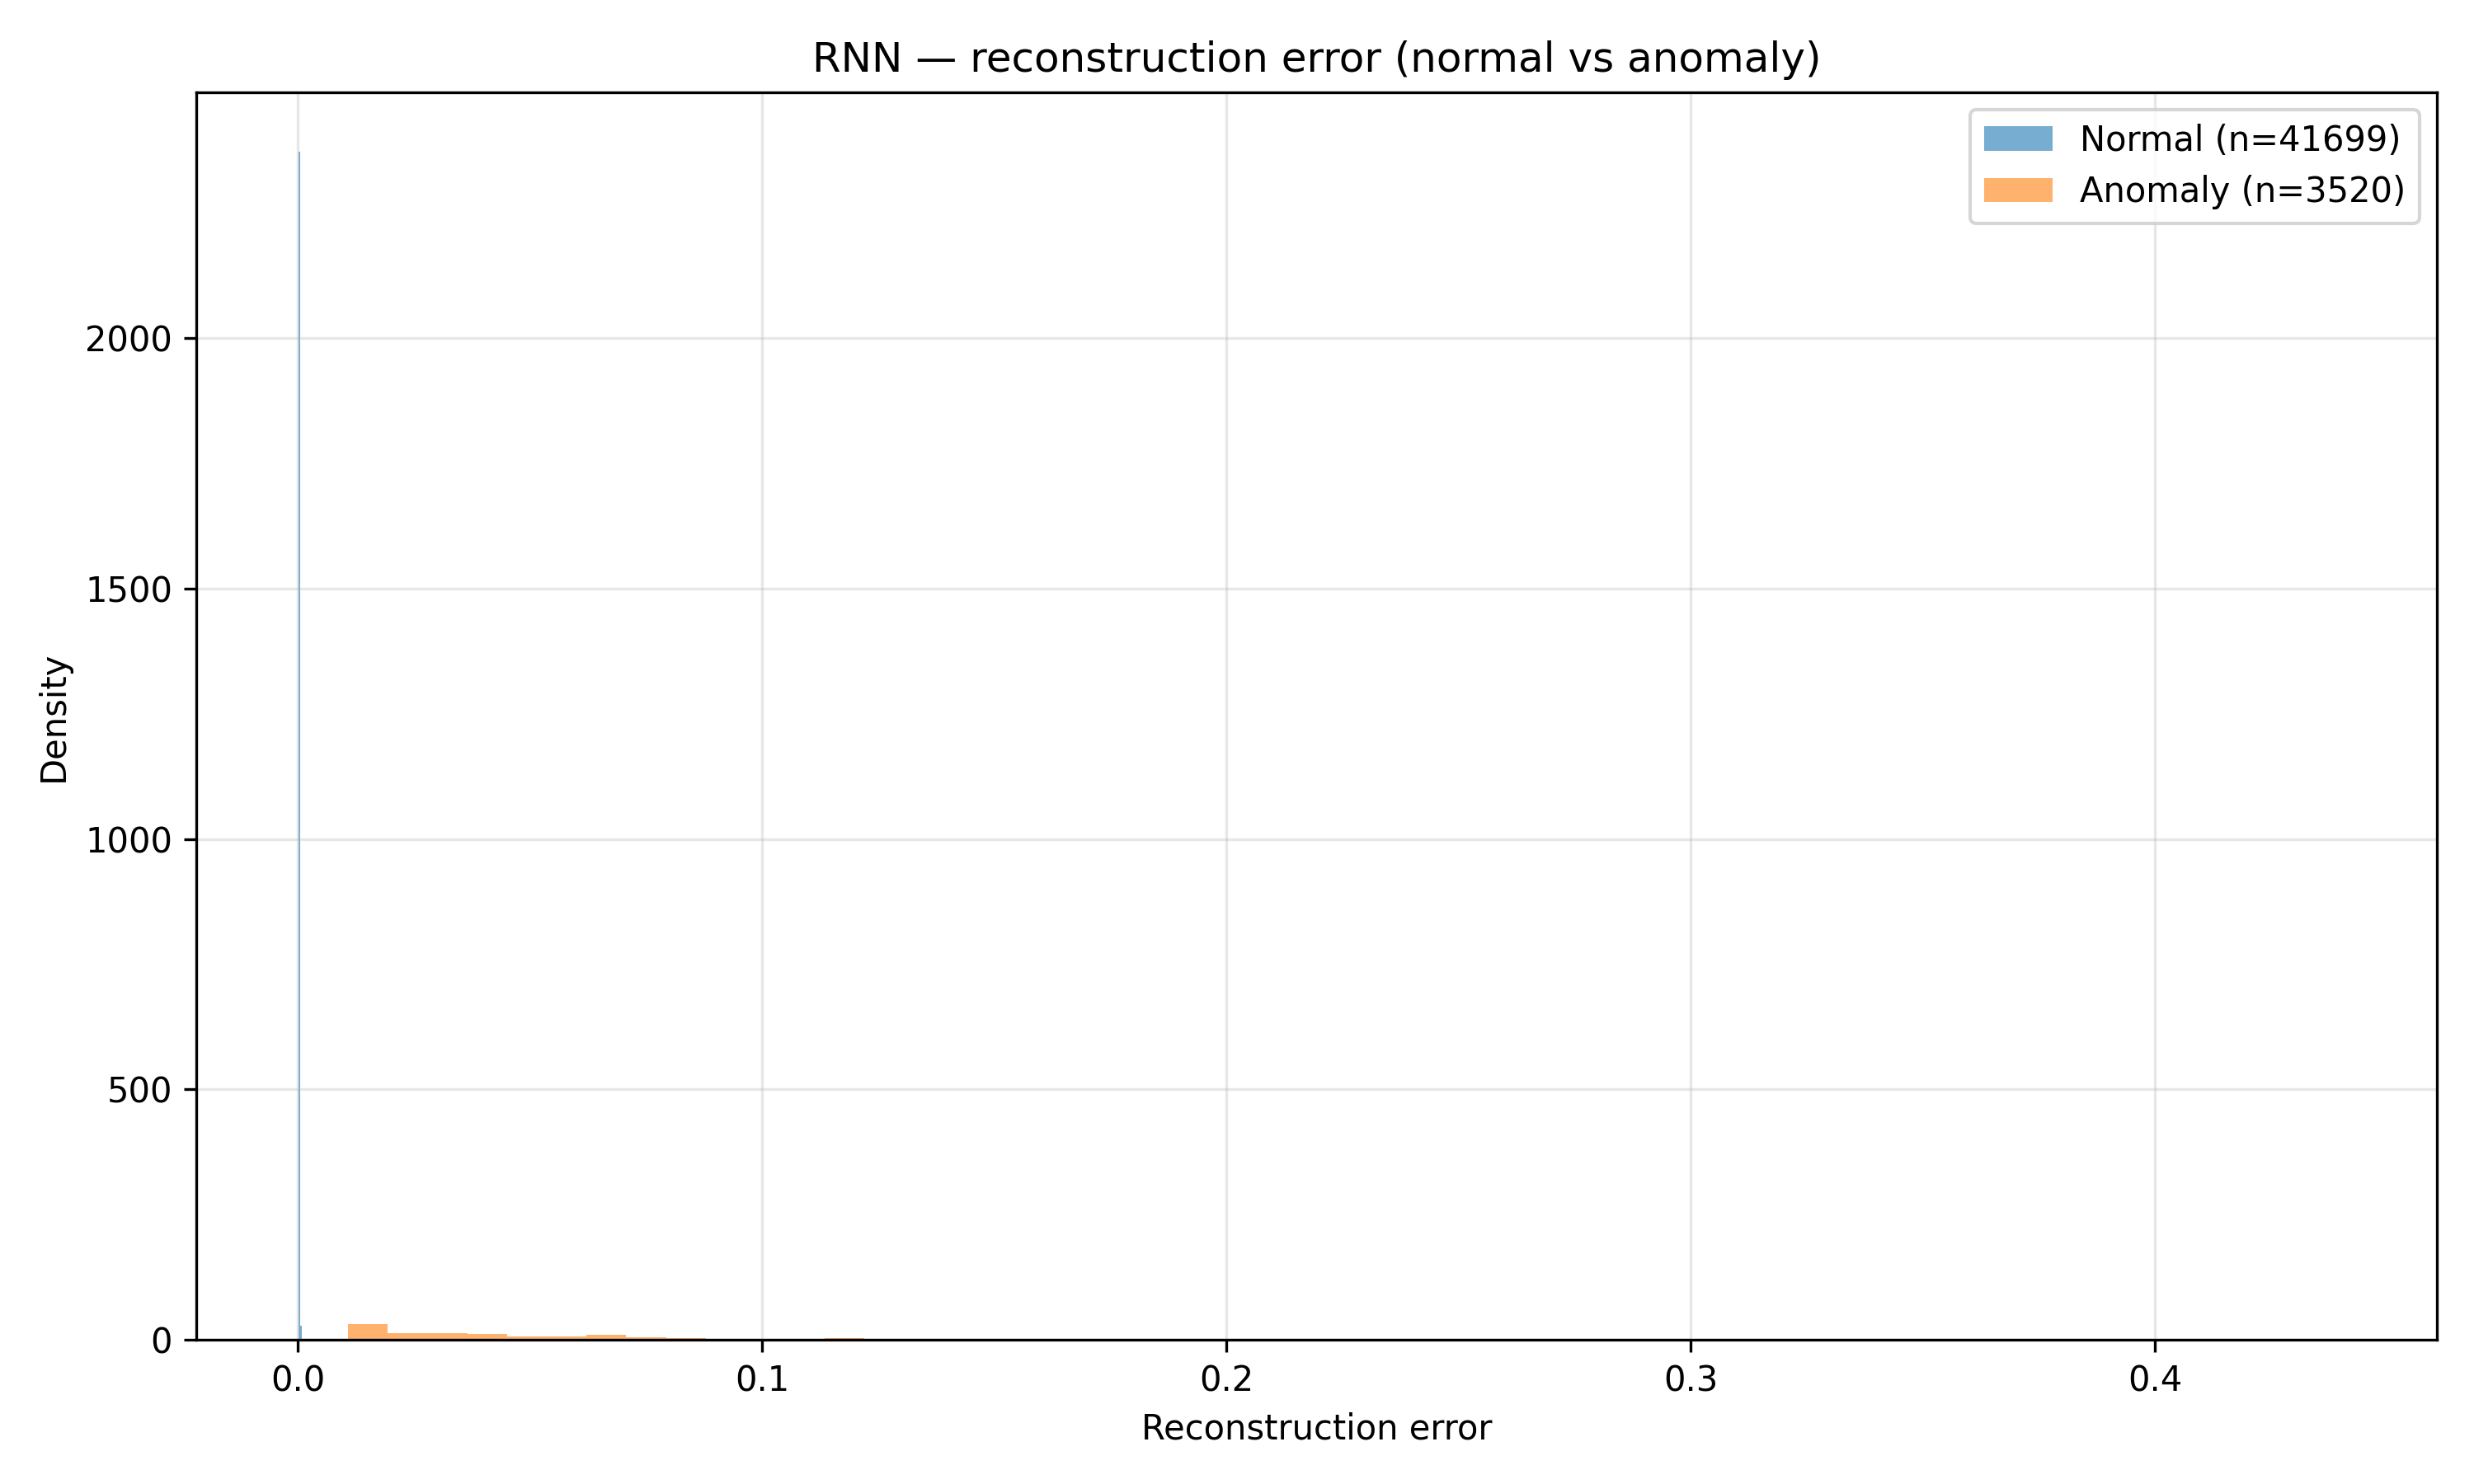
\includegraphics[scale=0.7]{inc/images/rnn_reconstruction_error}
    \caption{Распределение ошибки реконструкции для модели RNN-AE.}
    \label{fig:rnn_reconstruction_error}
\end{figure}

Для количественной оценки качества обнаружения аномалий используется метрика площади под PR-кривой (PR-AUC), которая особенно полезна при сильном дисбалансе классов.

На рисунке~\ref{fig:rnn_pr_curve} представлена PR-кривая для модели RNN-AE.

\begin{figure}
    \centering
    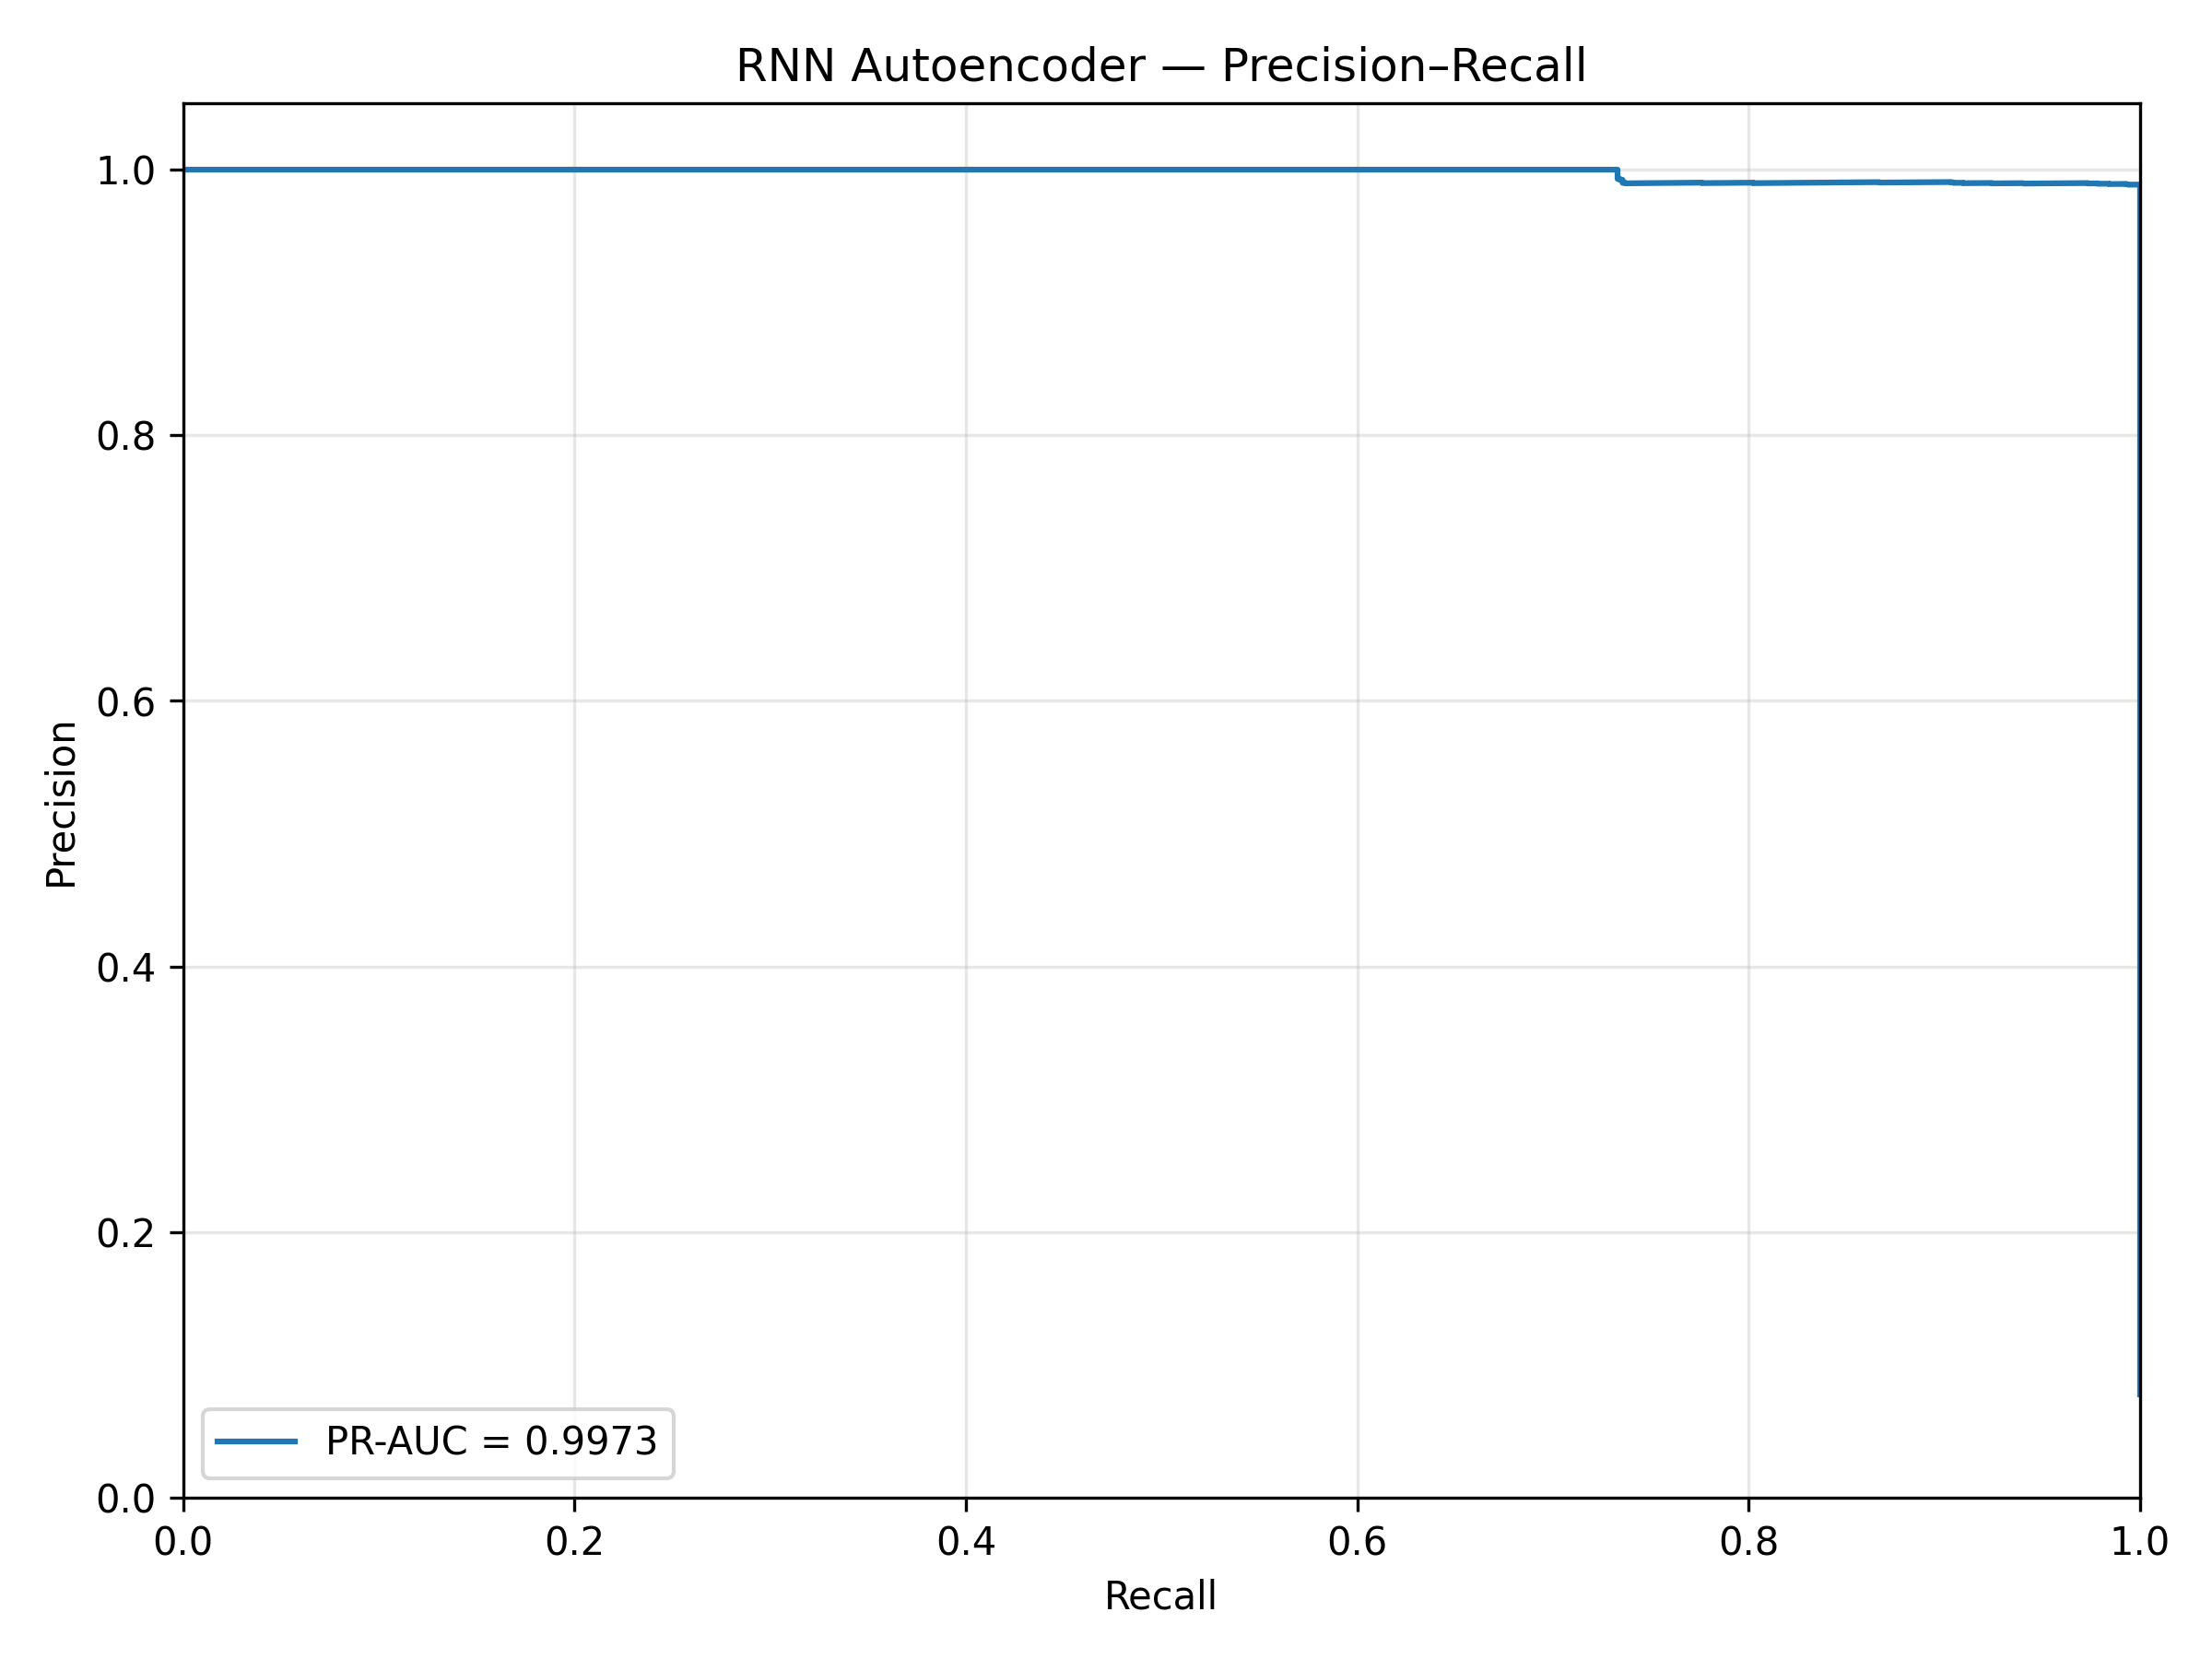
\includegraphics[scale=0.7]{inc/images/rnn_pr_curve}
    \caption{PR-кривая для модели RNN-AE.}
    \label{fig:rnn_pr_curve}
\end{figure}

\subsubsection{LSTM-Autoencoder}

В данной работе LSTM применяется в архитектуре \textit{autoencoder} (LSTM-AE), где слои \textit{encoder} и \textit{decoder} состоят из LSTM-блоков. Такая структура позволяет учитывать временную последовательность событий audit-логов и выявлять аномальные паттерны поведения пользователей и сервисных аккаунтов.

На рисунке~\ref{fig:LSTM-AE} приведена архитектура LSTM-AE, состоящая из двух частей:

\begin{itemize}
    \item \textbf{Encoder} — один или несколько LSTM-слоёв, преобразующих последовательность входных векторов $x_t$ в фиксированный вектор контекста $z$, содержащий сводную информацию о последовательности событий;
    \item \textbf{Decoder} — LSTM-слои, которые на основе вектора $z$ восстанавливают исходную последовательность событий $\tilde{x}_t$.
\end{itemize}

\begin{figure}
    \centering
    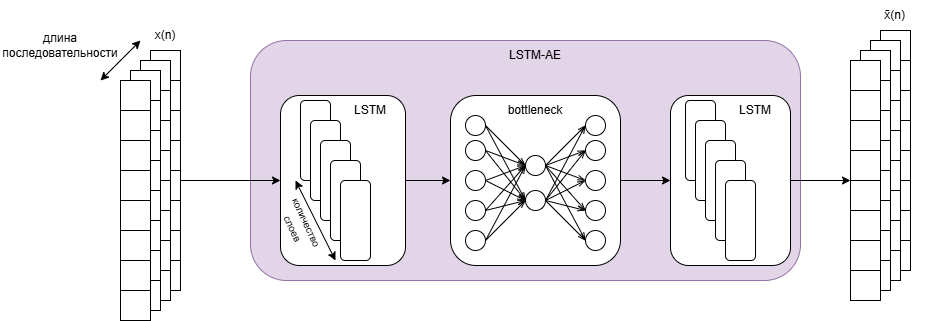
\includegraphics[scale=0.4]{inc/images/LSTM-AE-architecture}
    \caption{Архитектура LSTM-Autoencoder.}
    \label{fig:LSTM-AE}
\end{figure}

Функция потерь для обучения LSTM-AE определяется среднеквадратичной ошибкой, представленной в формуле~\ref{eq:lstm_mse}.
\begin{equation}\label{eq:lstm_mse}
    \mathcal{L}_{MSE} = \frac{1}{T} \sum_{t=1}^{T} \frac{1}{d} \| x_it - \tilde{x}_it \|_2^2
\end{equation}

где $T$ - длина последовательности, подающаяся в модель.

После обучения модели показатель аномальности вычисляется по формуле~\ref{eq:lstm_score}.

\begin{equation}\label{eq:lstm_score}
    s_t = \frac{1}{T} \sum_{t=1}^{T} \| x_it - \tilde{x}_it \|_2^2
\end{equation}

где $s_t$ — показатель аномальности для события $t$. События с $s_t$ выше порогового значения считаются аномальными.

На рисунке~\ref{fig:lstm_training_loss} приведён график изменения функции потерь LSTM-AE на обучающей и валидационной выборках.

\begin{figure}
    \centering
    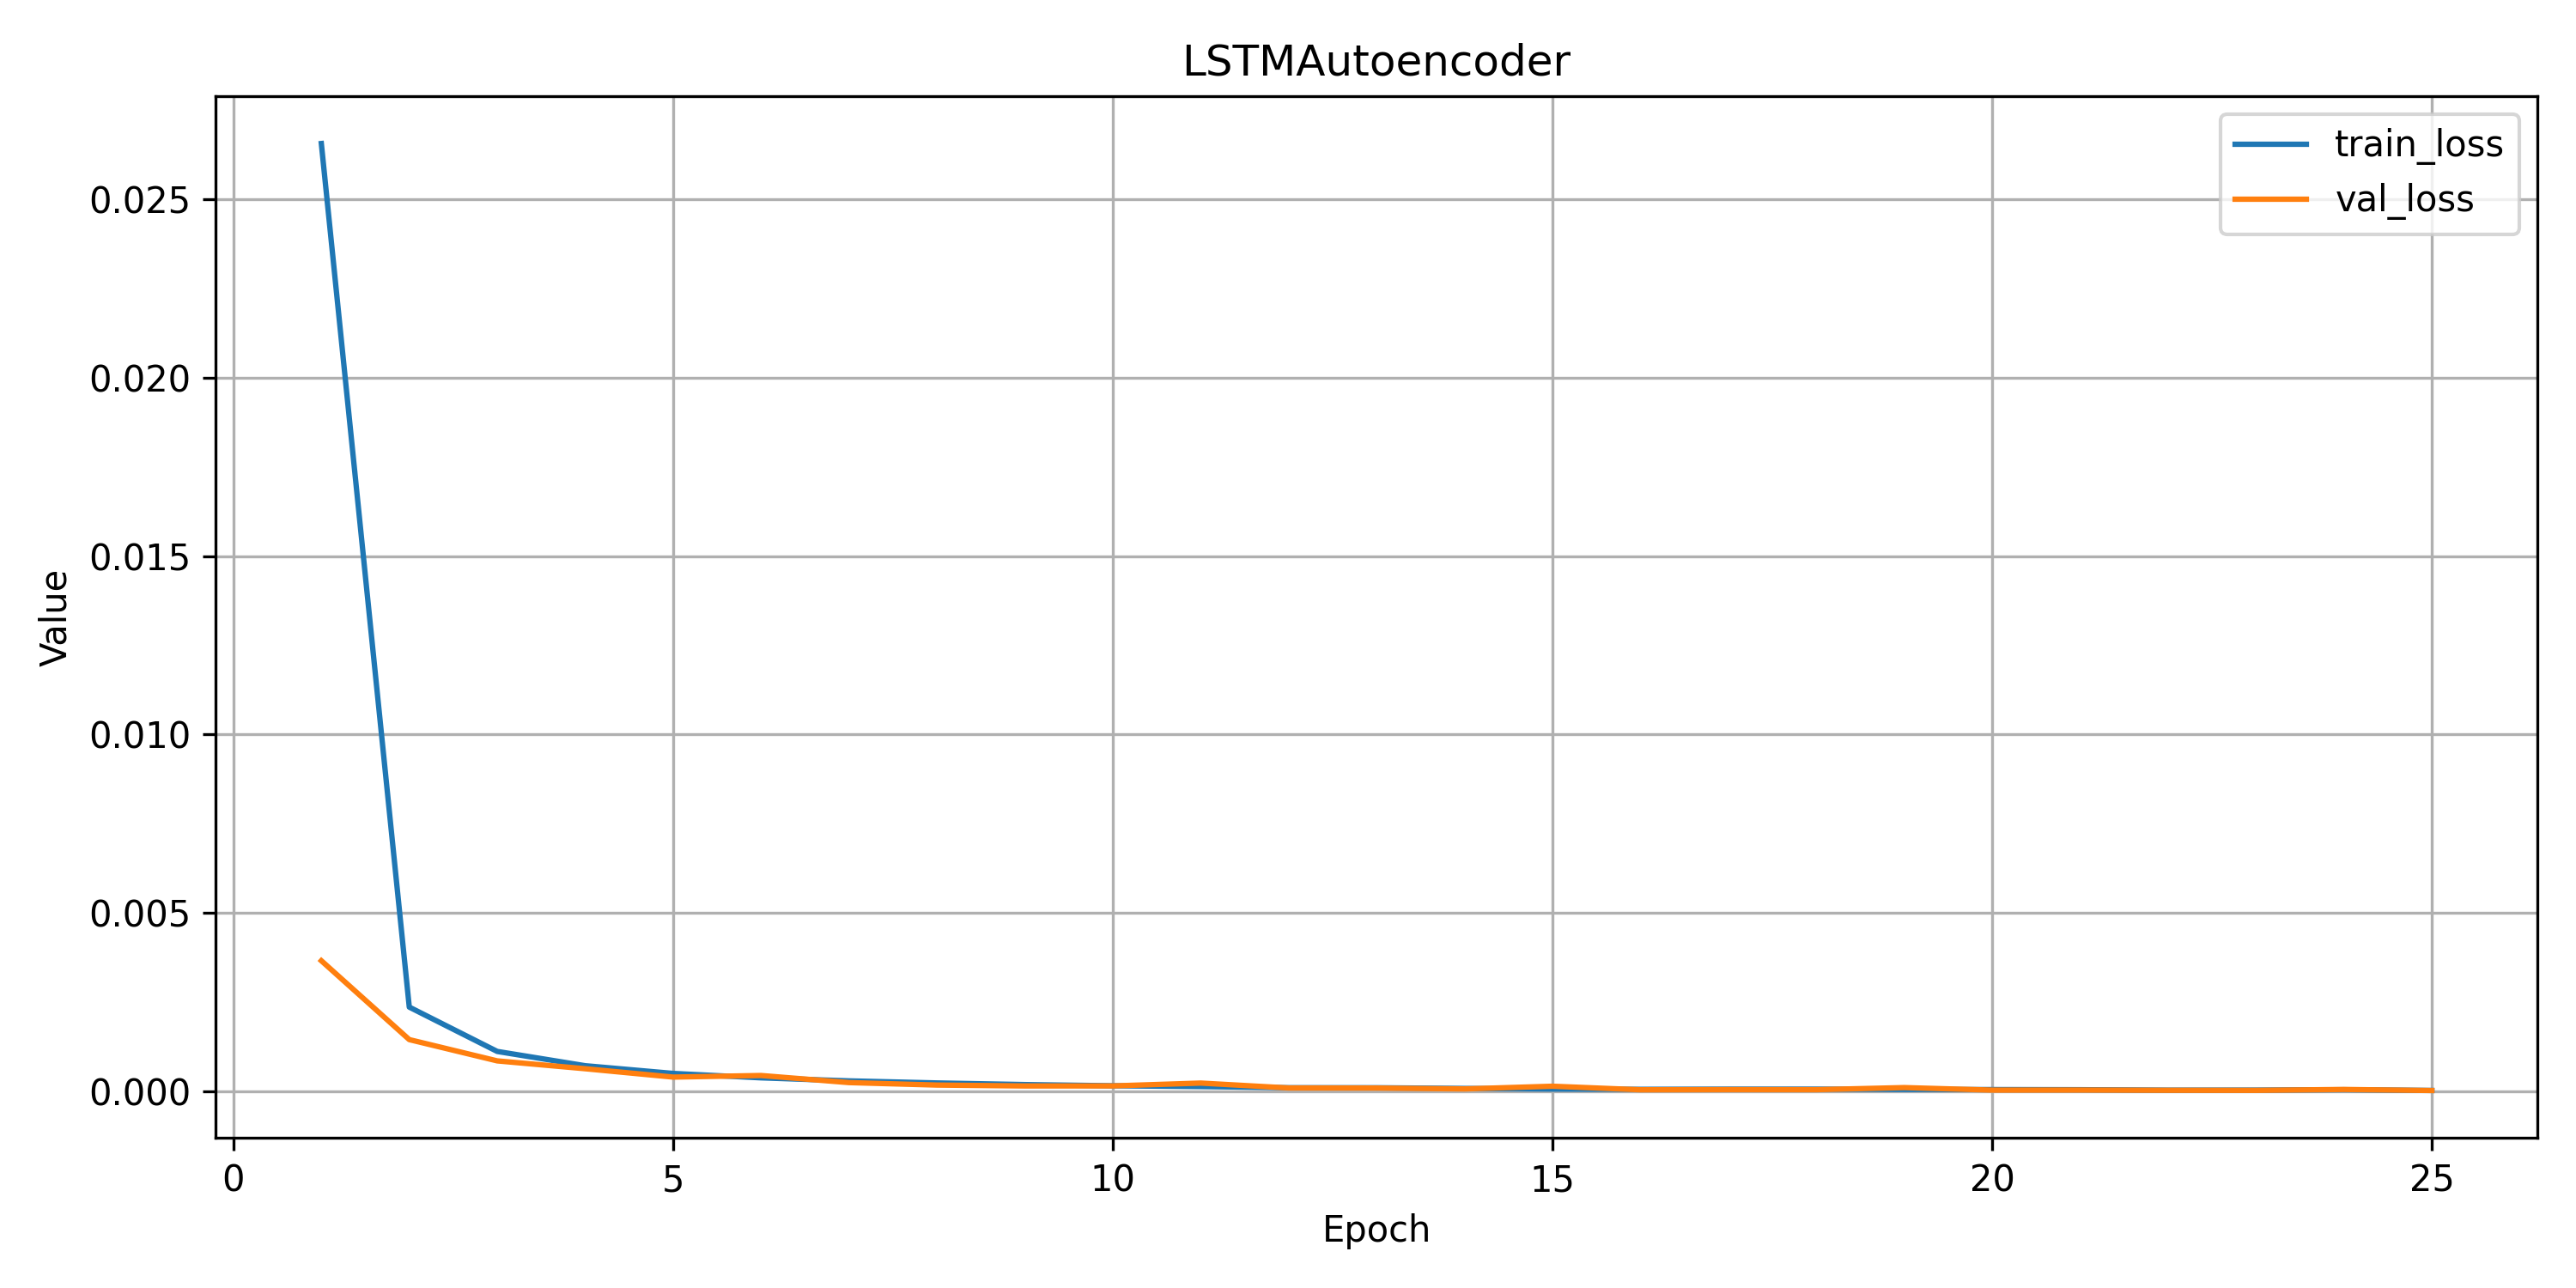
\includegraphics[scale=0.7]{inc/images/lstm_training_loss}
    \caption{Изменение функции потерь LSTM-AE на обучающей и валидационной выборках.}
    \label{fig:lstm_training_loss}
\end{figure}

После завершения обучения для каждого события тестовой выборки вычисляется показатель аномальности $s_t$, основанный на величине ошибки реконструкции.

На рисунке~\ref{fig:lstm_reconstruction_error} показано распределение ошибки реконструкции для нормальных и аномальных событий. Видно, что аномальные события обычно характеризуются более высокими значениями ошибки, что позволяет использовать этот показатель для их обнаружения.

\begin{figure}
    \centering
    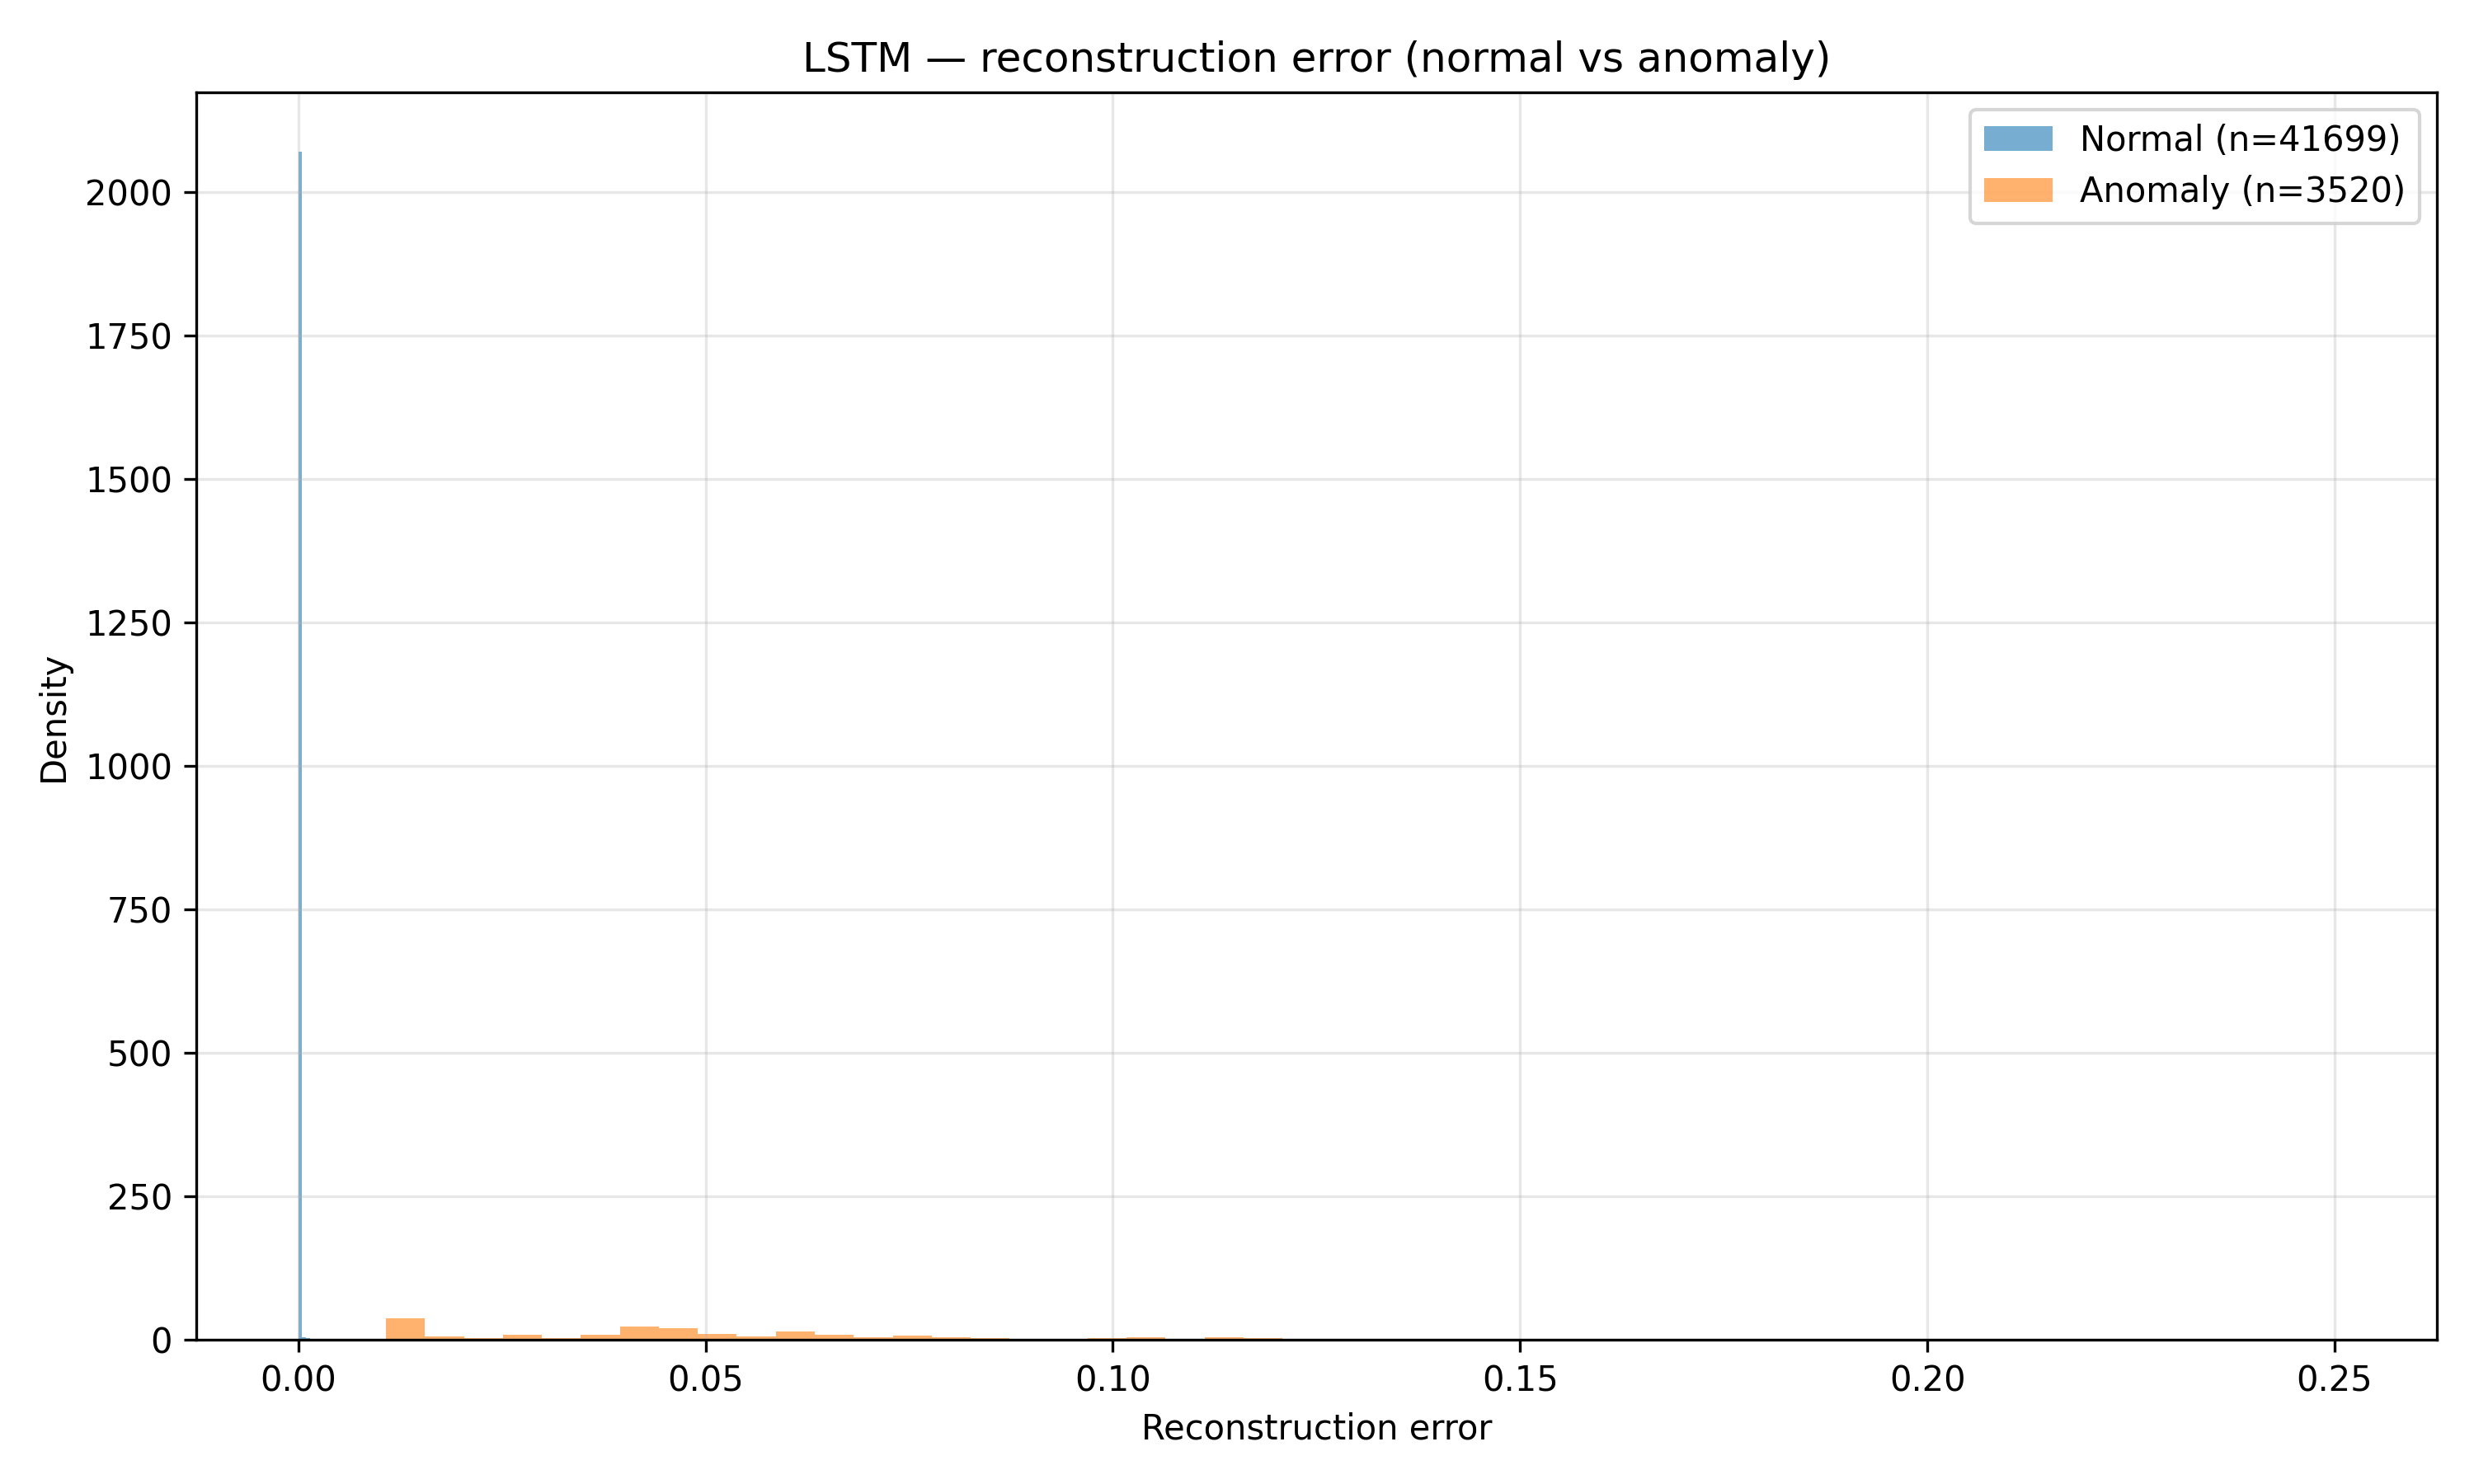
\includegraphics[scale=0.7]{inc/images/lstm_reconstruction_error}
    \caption{Распределение ошибки реконструкции для нормальных и аномальных событий.}
    \label{fig:lstm_reconstruction_error}
\end{figure}

На рисунке~\ref{fig:lstm_pr_curve} приведена PR-кривая, отражающая зависимость точности (Precision) от полноты (Recall) при изменении порога обнаружения.

\begin{figure}
    \centering
    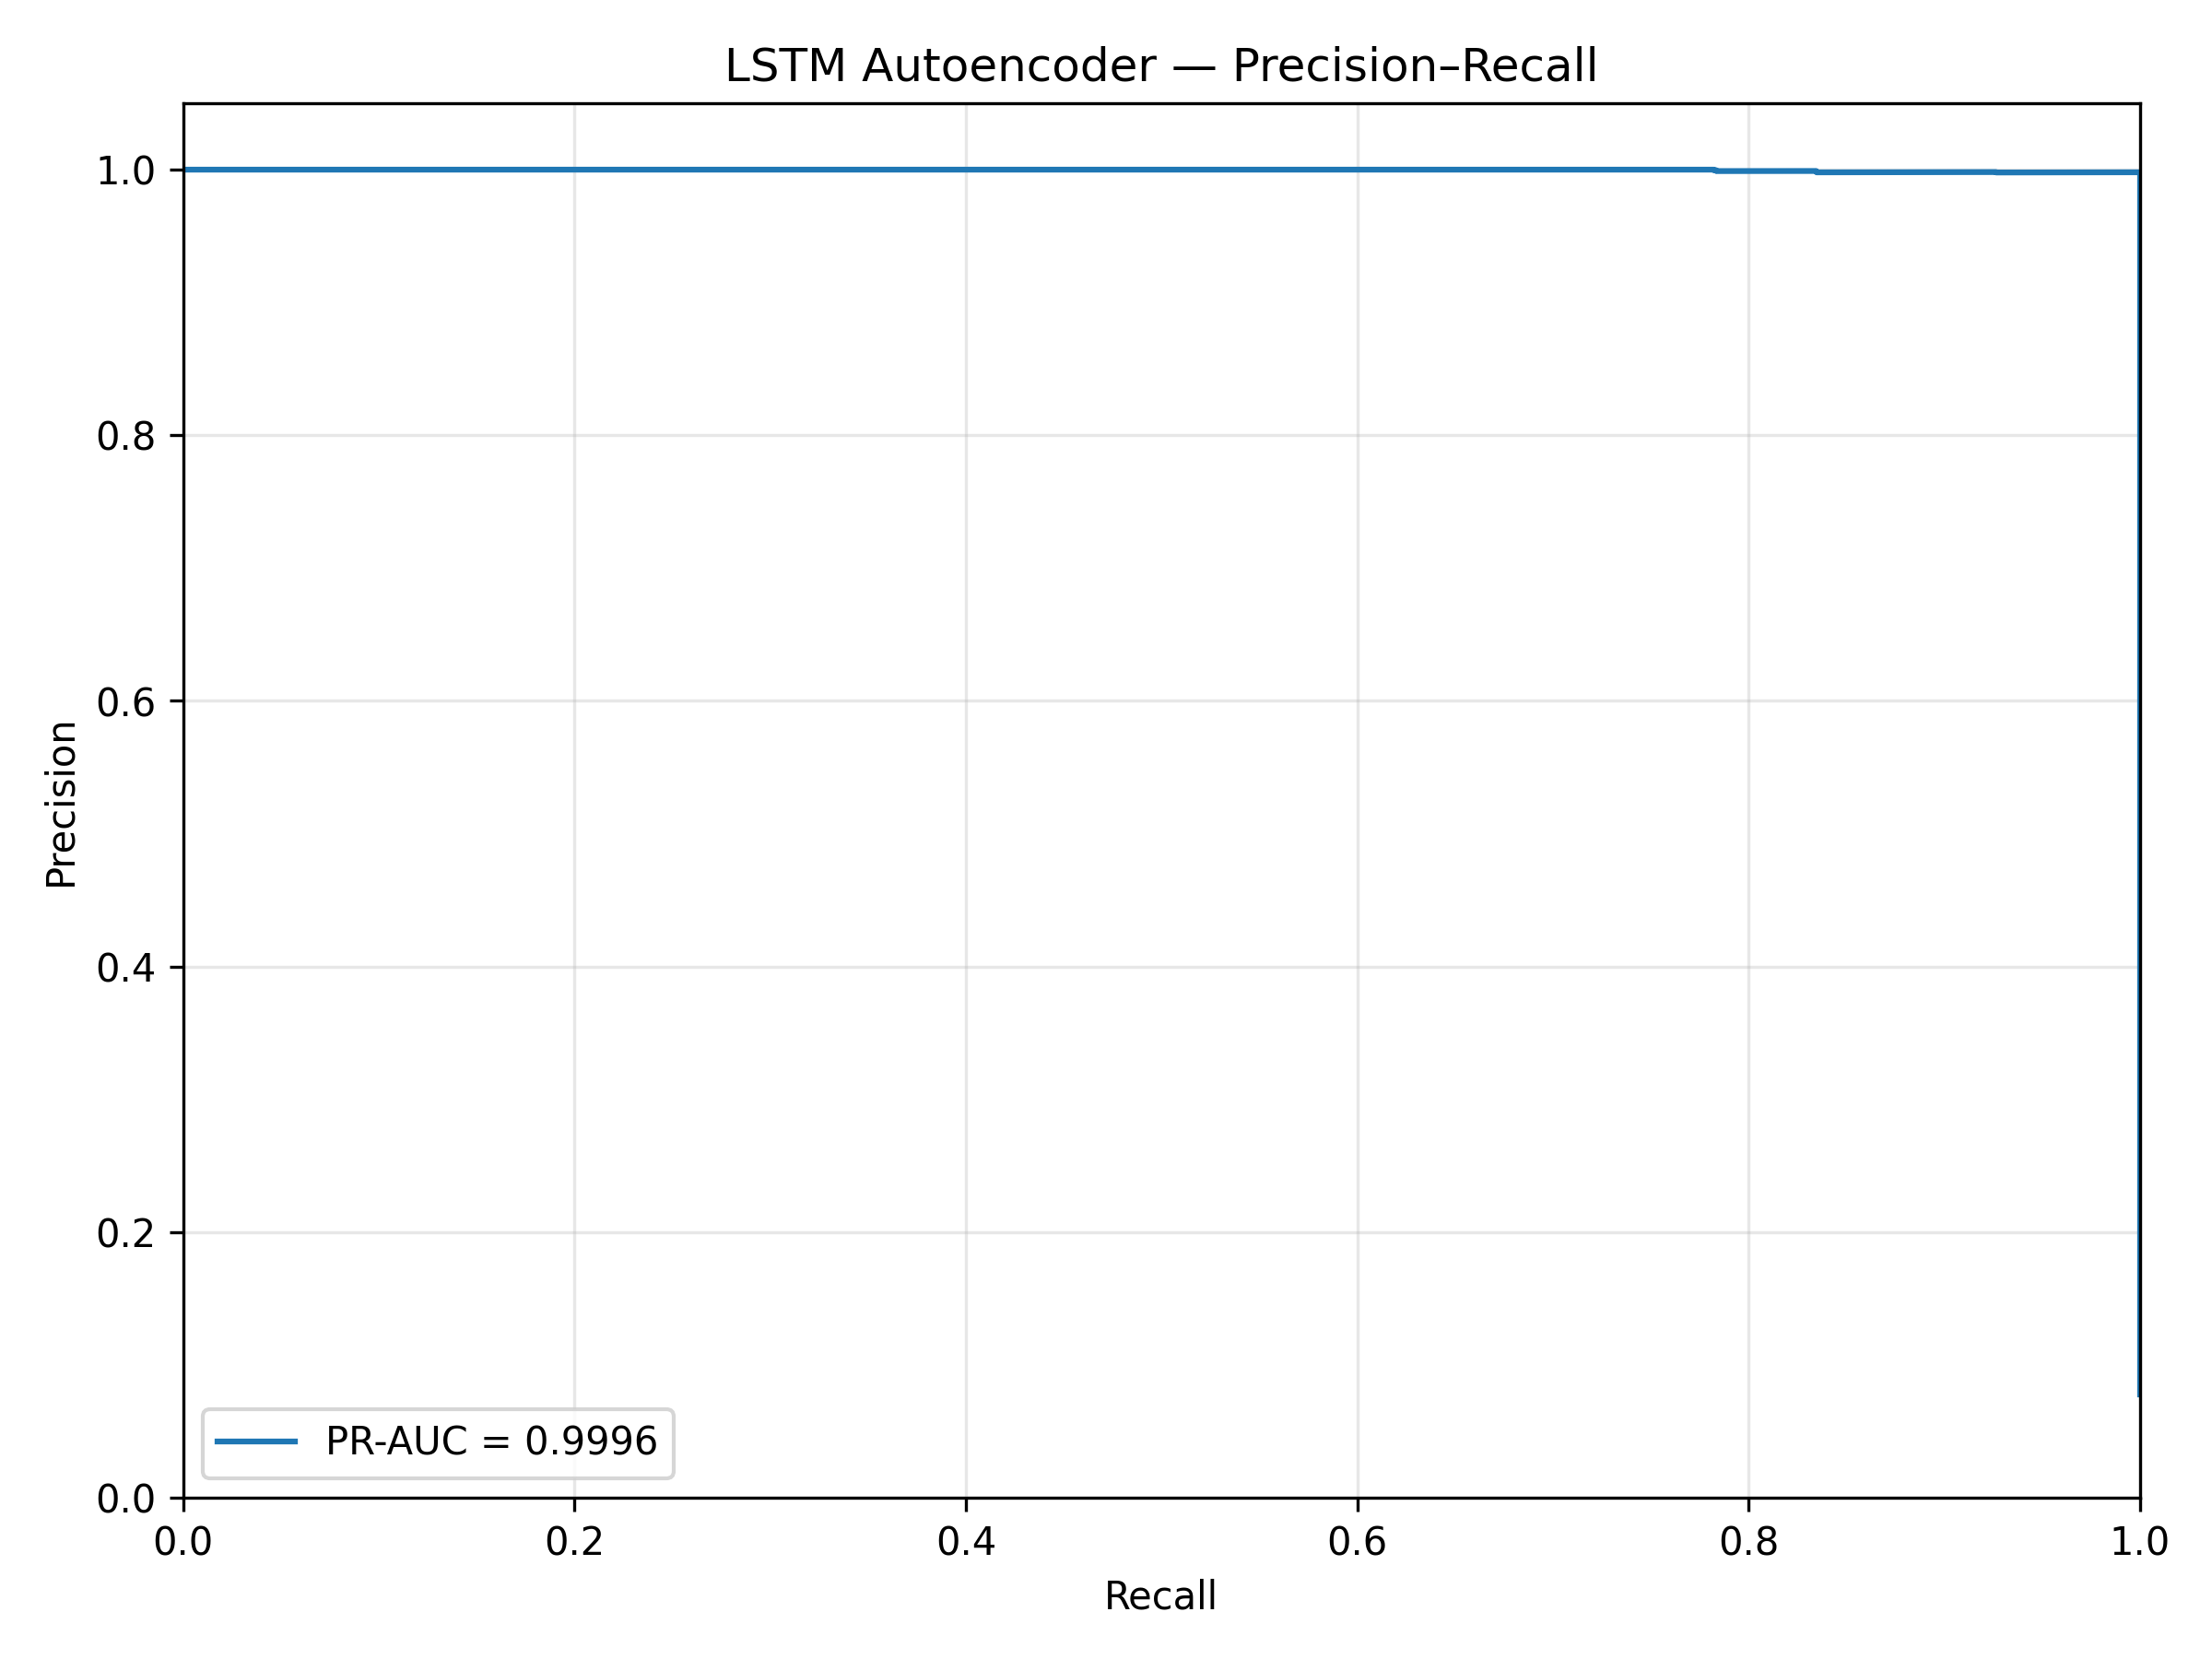
\includegraphics[scale=0.7]{inc/images/lstm_pr_curve}
    \caption{PR-кривая для модели LSTM-AE.}
    \label{fig:lstm_pr_curve}
\end{figure}

\subsection{Сравнительный анализ моделей и выбор оптимальной архитектуры}

После обучения моделей различных архитектур проводится их сравнительный анализ по метрикам качества обнаружения аномалий. Основной задачей данного этапа является определение архитектуры нейронной сети, обеспечивающей наилучшие результаты обнаружения аномалий на тестовой выборке.

Каждая модель обучалась на одинаковой обучающей выборке, содержащей преимущественно нормальные события, и оценивалась на тестовой выборке, включающей как нормальные, так и аномальные события.

В качестве основной метрики оценки качества использовалась площадь под кривой Precision--Recall (PR-AUC), которая является наиболее информативной при сильном дисбалансе классов, характерном для задачи обнаружения аномалий.

Дополнительно анализировались следующие метрики:

\begin{itemize}
    \item \textbf{ROC-AUC} — площадь под ROC-кривой;
    \item \textbf{Precision} — точность обнаружения аномалий;
    \item \textbf{Recall} — полнота обнаружения;
    \item \textbf{F1-score} — гармоническое среднее точности и полноты.
\end{itemize}

В таблице~\ref{tab:model_comparison} представлены результаты оценки моделей на тестовой выборке.

\begin{table}[h]
    \centering
    \caption{Сравнение моделей по метрикам качества}
    \label{tab:model_comparison}
    \begin{tabular}{|c|c|c|c|c|c|}
    \hline
    \textbf{Модель} & \textbf{ROC-AUC} & \textbf{PR-AUC} & \textbf{Precision} & \textbf{Recall} & \textbf{F1} \\
    \hline
    Autoencoder & 0.99988 & 0.99631 & 0.91394 & 1.00000 & 0.95503 \\
    \hline
    RNN-AE      & 0.99980 & 0.99733 & 0.93542 & 1.00000 & 0.96663 \\
    \hline
    LSTM-AE     & 0.99997 & 0.99962 & 0.93097 & 1.00000 & 0.96425 \\
    \hline
    \end{tabular}
\end{table}

Как видно из результатов, все модели демонстрируют высокое качество обнаружения аномалий. Однако между ними наблюдаются различия:

\begin{itemize}
    \item классический Autoencoder показывает наименьшее значение PR-AUC среди рассмотренных моделей;
    \item RNN-AE демонстрирует улучшение качества за счёт учета последовательной структуры данных;
    \item LSTM-AE достигает наилучшего значения PR-AUC и ROC-AUC, что свидетельствует о более точном разделении нормальных и аномальных событий.
\end{itemize}

Важно отметить, что все модели достигают максимального значения полноты (Recall = 1.0), что означает отсутствие пропущенных аномалий. При этом различия проявляются в количестве ложных срабатываний, отражаемых метрикой Precision.

На основании проведённого сравнительного анализа в качестве оптимальной модели была выбрана архитектура \textbf{LSTM-Autoencoder}.

Данный выбор обусловлен следующими факторами:
\begin{itemize}
    \item наивысшее значение PR-AUC, что критично для задач с дисбалансом классов;
    \item способность эффективно моделировать долгосрочные зависимости в последовательностях событий;
    \item более чёткое разделение распределений ошибки реконструкции для нормальных и аномальных событий.
\end{itemize}

Несмотря на то, что RNN-AE показывает сопоставимое значение F1-метрики, использование LSTM позволяет лучше учитывать сложные временные зависимости, характерные для audit-логов Kubernetes. Таким образом, LSTM-AE обеспечивает наилучший баланс между точностью обнаружения и устойчивостью модели, что делает её наиболее подходящей для практического применения в задаче обнаружения аномалий.